%%%%%%%%%%%%%%%%%%%%%%%%%%%%%%%%%%%%%%%%%%%%%%%%%%%%%%%%%%%%%%%%%%%%%%
% amspaper.tex --  LaTeX2e-based template for submissions to American 
% Meteorological Society Journals, including
%
% JAS 	-- Journal of the Atmospheric Sciences
% JAMC 	-- Journal of Applied Meteorology and Climatology
% JPO 	-- Journal of Physical Oceanography
% MWR 	-- Monthly Weather Review
% JTECH -- Journal of Atmospheric and Oceanic Technology
% WAF 	-- Weather and Forecasting
% JCLI 	-- Journal of Climate
% JHM 	-- Journal of Hydrometeorology
% JAM 	-- Journal of Applied Meteorology
%
% Template developed by B. Papa and S. Cooley, AMS. 
% Email questions to latex@ametsoc.org.
%
% August 12, 2008 (SRC)
%	- Clarified/added header notes, comments throughout
%	- Improved title page
%	- Edited text of document for clarity
%	- Altered list styles to adhere to AMS style, added comments
%	- Removed incorrect commands (i.e., \catcode) (corrects umlaut bug)
%	- Moved non-template commands to ametsoc.sty
%
% August, 2008 - B. Papa
% - Updated to handle two column journal page output
% - Updated text with new/modified instructions
%
% February, 2011 - B. Papa
% - Updated instructions for use with EM
%
% March, 2011 - B. Papa
% - Added use of \linenumbers
%
% July, 2012 - B. Papa
% - Updated instructions and text of document
%
%%%%%%%%%%%%%%%%%%%%%%%%%%%%%%%%%%%%%%%%%%%%%%%%%%%%%%%%%%%%%%%%%%%%%
% PREAMBLE
%%%%%%%%%%%%%%%%%%%%%%%%%%%%%%%%%%%%%%%%%%%%%%%%%%%%%%%%%%%%%%%%%%%%%
%
% The following three commands will generate a PDF that follows all the requirements for submission
% and peer review.  Uncomment these commands to generate this output (and comment out the two lines below.)
%
% DOUBLE SPACE VERSION FOR SUBMISSION TO THE AMS
\documentclass[12pt]{article}
\usepackage{ametsoc}
%\usepackage{ametsoc2col}
\linenumbers
%
% The following two commands will generate a single space, double column paper that closely
% matches an AMS journal page.  Uncomment these commands to generate this output (and comment
% out the two lines above. FOR AUTHOR USE ONLY. PAPERS SUBMITTED IN THIS FORMAT WILL BE RETURNED
% TO THE AUTHOR for submission with the correct formatting.
%
% TWO COLUMN JOURNAL PAGE LAYOUT FOR AUTHOR USE ONLY
%%%%%\documentclass[10pt]{article}
%%%%%\usepackage{ametsoc2col}
%
%%%%%%%%%%%%%%%%%%%%%%%%%%%%%%%%%%%%%%%%%%%%%%%%%%%%%%%%%%%%%%%%%%%%%
% ABSTRACT
%
% Enter your Abstract here
%%%%%%%%%%%%%%%%%%%%%%%%%%%%%%%%%%%%%%%%%%%%%%%%%%%%%%%%%%%%%%%%%%%%%
\newcommand{\myabstract}{The capability of the precipitation data assimilation is added to the data assimilation system for Weather Research and Forecasting model using four-dimensional variational data assimilation approach. The precipitation data used in this study is derived from National Center for Environmental Prediction Stage IV multi-sensor precipitation analyses.
Four experiments over a 1-month period in June 2010 are conducted to assess the impact of precipitation assimilation on analyses and short-range forecasts, and the results for a single weather event in this period are presented to further investigate this impact. 
Results show that the assimilating precipitation has a positive impact on model fields, particularly on the low level humidity. For the impact on precipitation forecasts, it indicates that precipitation assimilation succeeded in bringing the model precipitation closer to the observations through the changes in temperature, moisture and wind imposed in the analyses.}
%
\begin{document}

%
%%%%%%%%%%%%%%%%%%%%%%%%%%%%%%%%%%%%%%%%%%%%%%%%%%%%%%%%%%%%%%%%%%%%%
% TITLE
%
% Enter your TITLE here
%%%%%%%%%%%%%%%%%%%%%%%%%%%%%%%%%%%%%%%%%%%%%%%%%%%%%%%%%%%%%%%%%%%%%
\title{\textbf{\large{The impact of assimilating NCEP Stage IV Precipitation on analyses and short-range forecasts in WRFDA 4D-Var}}}
%
% Author names, with corresponding author information. 
% [Update and move the \thanks{...} block as appropriate.]
%

\author{\textsc{Junmei Ban, Xin Zhang}
            \thanks{\textit{Corresponding author address:} 
            Dr. Xin Zhang, National Center for Atmospheric Research, 
            P. O. Box 3000, Boulder, CO 80307. 
            \newline{E-mail: xinzhang@ucar.edu}}\quad\textsc{and Xiang-Yu Huang}\\
\textit{\footnotesize{National Center for Atmospheric Research, Boulder, Colorado 80307, USA}}
}

%
% The following block of code will handle the formatting of the title page depnding on whether
% we are formatting a double column (dc) author draft or a single column paper for submission.
% AUTHORS SHOULD SKIP OVER THIS... There is nothing to do in this section of code.
\ifthenelse{\boolean{dc}}
{
\twocolumn[
\begin{@twocolumnfalse}
\amstitle

% Start Abstract (Enter your Abstract above.  Do not enter any text here)
\begin{center}
\begin{minipage}{13.0cm}
\begin{abstract}
	\myabstract
	\newline
	\begin{center}
		\rule{38mm}{0.2mm}
	\end{center}
\end{abstract}
\end{minipage}
\end{center}
\end{@twocolumnfalse}
]
}
{
\amstitle
\begin{abstract}
\myabstract
\end{abstract}
\newpage
}
%%%%%%%%%%%%%%%%%%%%%%%%%%%%%%%%%%%%%%%%%%%%%%%%%%%%%%%%%%%%%%%%%%%%%
% MAIN BODY OF PAPER
%%%%%%%%%%%%%%%%%%%%%%%%%%%%%%%%%%%%%%%%%%%%%%%%%%%%%%%%%%%%%%%%%%%%%
%
\section{Introduction}

In the past few decades, several approaches to assimilation of precipitation observations in NWP models have been developed
to improve the model initial states, and hence, to improve the skill of short-range forecasts.

The first approach is initialization scheme (or �reverse� scheme), such as dynamical initialization \citep{Fiorino}, physical initialization  \citep{Krishnamurti} and cumulus convection initialization  \citep{Kasahara,Donner}. The basic idea of these methods is to restructure the moisture and temperature fields so that they are consistent with observed precipitation rates. The papers mentioned above all showed that an improved forecast could be obtained after incorporation of the observed rainfall rate. However, this is an indirect way of using precipitation data, and the shortcoming of the technique is that it does not guarantee dynamically consistent initial conditions \citep{Zou}.

The second method is to use nudging techniques \citep{Carr,Kuo1993,Lin,Macpherson}.  \cite{Carr} use precipitation data during continuous FDDA (Four-Dimensional Data Assimilation) via a nudging technique. In 2001 the nudging of precipitation observations \citep{Lin} was included in the Eta Data Assimilation System (EDAS). Meanwhile, \cite{Macpherson} implemented the latent heat nudging technique to incorporate radar-derived rainfall data into the Met office operational mesoscale model. Although it is one of the simplest methods of data assimilation and computationally much more economical, the nudging-generated initial conditions, like the first method, are also dynamically inconsistent \citep{Zou,Bao}.

The third approach is to use variational data assimilation, such as, 1D-Var, 3D-Var, 1D-Var+4D-Var, and 4D-Var. We will not go into many details about 1D-Var and 3D-Var assimilating rainfall data, and more information can be found in the following papers (1D-Var: \citet{Hou}; 3D-Var: \citet{Treadon}). \cite{Zupanski} demonstrated the technical feasibility of the approach, and showed an improvement of precipitation forecasts in the mid-latitudes by using a regional National Meteorological Center (NMC) eta forecast model and an incomplete adjoint model. Later, studies \citep{Zou,Xiao,Guo,Zhangandliu,Xu} indicated that the precipitation assimilation using the fifth-generation Mesoscale Model (MM5) 4D-Var leads to a reduction in spin-up time, improves the moisture distributions in model initial conditions and improves the skill of short-range forecasts. 

Some operational weather services also assimilate precipitation operationally using 4D-Var method to improve precipitation forecasts, including the Japan Meteorological Agency (JMA) \citep{Koizumi} and the European Centre for Medium-Range Weather Forecasts (ECMWF)  \citep{Lopez}. Koizumi et al. (2005) reported that JMA implemented a mesoscale four-dimensional variational assimilation system (Meso 4D-Var) to assimilate precipitation data. They reported the precipitation forecast  throughout the 18-hour forecast time have been improved, although Meso 4D-Var does not include the adjoint codes of cumulus parameterization. \citet{LopezandBauer}, employed 1D+4D-Var approach to assimilate National Center for Environmental Prediction(NCEP) Stage IV precipitation estimates at ECMWF. In the first step, temperature and specific-humidity profiles are retrieved from surface rainfall-rate observations via a 1D-Var approach. In the second step, the total column water vapor derived from the 1D-Var humidity profiles is assimilated in 4D-Var. This means that the rainfall-rate information is first converted into humidity information before being used in 4D-Var. In 2011, Lopez reported that the direct 4D-Var assimilation of NCEP Stage IV data has been developed and tested in ECMWF's global Integrated Forecasting System. Compared to the initialization scheme, 4D-Var can assimilate precipitation data directly, and the major advantage of 4D-Var is that it uses the full model dynamics to adjust the model variables to the observed precipitation \citep{Tsuyuki}.

In this study, precipitation assimilation capability is added into the WRF Data Assimilation System (WRFDA) 4D-Var \citep{Barker,Huang,Zhang}. 
The WRF model's tangent linear (TLM) and adjoint model (ADM) used here has been redeveloped by \citet{Zhang} and it contains a simplified cumulus parameterization and large-scale condensation.
The purpose of this study is to assimilate precipitation observations in WRFDA 4D-Var and explore the impact of precipitation assimilation on analyses and subsequent forecasts. Four experiments have been conducted over a 1-month period from 1 to 30 June 2010. Observations used in assimilation  experiments are conventional data and NCEP Stage IV 6-hourly accumulated precipitation. The results are evaluated using the Model Evaluation Tool (MET) which was developed at National Center for Atmospheric Research (NCAR) Developmental Testbed Center (DTC)\citep{Brown} .
The outline of the paper is as follows: 
The data used in assimilation experiments are described in section 2. WRFDA 4D-Var is described in section 3. Experiments design and verification methods are introduced in Section 4.  In Section 5 and 6, we present 1-month average results and a single case study respectively. The conclusion is given in Section 7.

\section{Observations}
The set of precipitation observations to be assimilated in this paper is NCEP Stage IV precipitation data, 
which is based on the multi-sensor (radar and gauges) hourly/6-hourly NCEP Stage III analyses produced by the 12 River Forecast Centers (RFCs) in continental United States (CONUS) and benefits from the RFCs� manual quality control step. 
The Stage IV analysis is used at NCEP as input for precipitation assimilation in the Eta model, as part of the forcing for the land surface model, and as verifying analyses in precipitation forecast verification \citep{LinMitchell}. 
Hourly, 6-hourly and 24-hourly precipitation data are available on the National Center for Atmospheric Research (NCAR) Cooperative Distributed Interactive Atmospheric Catalog System (CODIAC) (http://data.eol.ucar.edu/codiac/dss/id=21.093). 
We choose 6-hourly precipitation data  instead of hourly for 6-hour assimilation window to better satisfy the 4D-Var linearity assumption \citep{Lopez}. The 6-hourly precipitation observations have been converted into WRFDA-readable data format and the precipitation error is assigned a value of 5 mm, which will be discussed in more detail in section 6c. Original 4km resolution data are thinned to the experiment's resolution of 30km. 

Conventional data used in this paper includes land surface, marine surface, radiosonde, pibal and aircraft reports from the Global Telecommunications System (GTS) which originated from a wide variety of sources, and it was downloaded from http://rda.ucar.edu/datasets/ds337.0/ . 

\section{A brief description of WRFDA 4D-Var}

 \citet{Huang} described the formulation of the WRFDA 4D-Var system and presented preliminary results from real-data 4D-Var experiments. The system consisted of WRF-Var, WRF and WRF+ (TLM and ADM) and was compiled as multiple executables. Later, WRF TLM and ADM (called WRFPLUS) was redeveloped by \citet{Zhang} based on the latest repository WRF. Simplified large-scale condensation and cumulus schemes are included in WRFPLUS, which makes it possible to add the function of assimilating precipitation data in WRFDA 4D-Var.
 
The objective of 4D-Var is to find the optimal estimate of the true atmospheric state at the analysis time by iteratively minimizing a cost function which can be written as,\begin{align}
J &= \frac{1}{2}\ (x^{n}-x^{b})^{T}\mathbf{B}^{-1} (x^{n}-x^{b})\nonumber\\
& + \frac{1}{2}\sum_{k=1}^{K}(\mathbf{H}_k\mathbf{M}_k (x^{n}-x^{n-1}) - d_{k})^{T}\mathbf{R}^{-1}(\mathbf{H}_k\mathbf{M}_k (x^{n}-x^{n-1}) - d_{k})  
\end{align}

where $J$ is a quadratic measure of distance between (i) the analysis and the background, and (ii) the analysis and the observations. In the background term, $ {x}^{n} $ is the analysis vector of model control variables at the nth outer loop, $ {x}^{b} $ is the background. $ \mathbf{B} $ is a covariance matrix for background error,  which is computed using the NMC method \citep{ParrisDerber}. 
In the observation term, $K$ is the total number of time slots in which observations are available. $ \mathbf{H} $ is the linearized observation operator which transforms variables from gridded analysis space to observation space. $ \mathbf{M} $  is the tangent linear model. $ {x}^{n-1} $ is the analysis vector from the previous outer loop. $ d_{k} $ is the innovation vector given by $ d_{k}=H_k\left[M_k(x^{n-1})\right]-y_{k}$. $H$ and $M$ are the nonlinear observation operator and simplified WRF nonlinear model, respectively. $ \mathbf{R} $ is the observation error covariance matrix. 
The conjugate gradient method is used to minimize the cost function. 

It should be noticed that assimilation of precipitation observations is different from  conventional data assimilation in the following ways: Firstly, rain gauge observations are total amounts, which can include large-scale and/or convective precipitation in a model simulation. Secondly,  precipitation is not included as a control variable, but the assimilation of precipitation observations will have feedback to all the control variables via the adjoint of the physics package. Moreover, the model precipitation is an integral quantity and the same duration of model precipitation should be compared to the observations \citep{Zupanski,Zou}.

\section{Experiments design and verification methods}
\subsection{Experiments design}

The Advanced Research Weather Research and Forecasting model (ARW-WRF) \citep{Skamarock} is used as the forecast model. The integration domain of the model covers the North American continent and the surrounding oceans. The horizontal resolution is 30km and there are 40 vertical levels with the model top at 50hPa. The WRF Single-Moment 5-class Microphysics scheme (WSM5)  \citep{Hong}, the Kain-Fritsch cumulus convection scheme \citep{KainFristsch}, and the Yonsei University (YSU) boundary layer parameterization \citep{Hong2006} are used. 

Four experiments, CONTROL, GTS, RAIN and GTS+RAIN, were performed from 0000 UTC 1 to 1800 UTC 30 June 2010.  
A 6-h spin-up run is conducted at four analysis times (0000, 0600, 1200, and 1800 UTC) every day using NCEP Final Analysis (FNL) with horizontal spatial resolution of 1.0 x 1.0 degree and the output from the spin-up is used as the initial condition of the CONTROL experiment as well as the first guess field for the 4D-Var experiments. The CONTROL run is performed without data assimilation and serves as the benchmark for evaluating the assimilation experiments. The GTS experiment only assimilates conventional observations, while the RAIN experiment only assimilates precipitation data. The GTS+RAIN experiment assimilates both conventional and precipitation data.  
The NMC method \citep{ParrisDerber} in the WRFDA package is used for background error calculations. 
To reduce the computational cost, multi-incremental 4D-Var is used, where the innovation in the outer loop is computed with a high-resolution nonlinear model (30 km) and the minimization in the inner loop is done with a low-resolution linearized model (90 km). A more detailed description of multi-incremental 4D-Var can be found in \cite{Zhangandhuang}. 

\subsection{Verification methods}

The MET developed at NCAR DTC is used to evaluate the analyses and forecasts. Two datasets have been used as references. One dataset is the upper air sounding observations, which is used to evaluate model winds, temperature, and relative humidity. Root-mean square errors (RMSEs) are used as the verification metric. The other dataset is the NCEP Stage IV precipitation data. The original precipitation accumulations are available on a 4-km resolution polar-stereographic grid. It has been regrided to 30 km lambert conformal grid before verification. We acquire 12-h, 18-h and 24-h accumulated precipitation by summing of NCEP Stage IV 6-h accumulated precipitation. After interpolating and summing, verifications are done by using a grid-to-grid comparison. The Gilbert Skill Score (GSS) \citep{Gilbert} is used as the precipitation verification metric. RMSEs and GSSs have been calculated for the entire 1-month period of the experiments. Statistical significance was assessed by applying a bootstrap resampling technique.

\section{1-month averaged results} 

\subsection{Impact on model varisables}
In order to evaluate how model variables are affected by the precipitation assimilation, RMSEs are computed for wind speed, temperature and relative humidity on different pressure levels.  Figure 1 gives the vertical profiles of wind speed RMSEs for four experiments at analysis, 12-h and 24-h forecast. The confidence intervals were added to help visualize the uncertainty, and the horizontal bars represent the confidence intervals at the 95\% confidence level. At analysis time (Figure 1a), the RMSE of CONTROL is between 2.5 m s$^{-1}$ and 4 m s$^{-1}$ from 1000hpa to 100hpa. GTS has statistically significant lower RMSE than CONTROL in all levels and the largest RMSE difference between them is about 0.9 m s$^{-1}$ at 200hpa.   For the RAIN experiment, the RMSE is close to CONTROL except at lower level where RAIN gives smaller error of about 2.2 m s$^{-1}$.  It indicated that only assimilating precipitation data can reduce the lower level RMSE, but the influence to higher level is very  neutral. The wind speed RMSE of GTS+RAIN is almost overlapped with GTS at analysis time. It suggested that the conventional data play a dominate role in improving the vertical structure of the wind speed fields in GTS+RAIN at analysis time. For 12-h and 24-h forecasts (Figure 1b and 1c), although the wind speed RMSE of the four experiments are very close, the RMSEs of GTS+RAIN are smaller than other experiments almost at all levels. 

The vertical profiles of the temperature RMSEs for all experiments are shown in Figure 2. Comparing to CONTROL, the RMSEs in GTS and GTS+RAIN have been statistically significant reduced at all levels for analyses (Figure 2a). RAIN has smaller RMSE than CONTROL at 1000hpa for analysis, and the confidence intervals indicated that the differences are statistically distinct at this level. The temperature RMSEs for 12-h and 24-h forecasts obtained by four experiments are similar: the confidence intervals overlap each other. 

The vertical profiles of the relative humidity RMSEs for all experiments are shown in Figure 3.  Unlike wind speed and temperature fields, GTS+RAIN have not overlapped with GTS at analysis time, and the confidence intervals show that GTS+RAIN reduced RMSE significantly compared to GTS and CONTROL at 1000hpa. At 12-h forecast, GTS+RAIN still show an advantage of reducing low level RMSE. At 24-h forecast, the RMSE in GTS+RAIN is smaller than other experiments on the whole, but the differences are not significant. The positive impact on moisture field in precipitation assimilation is very important, for it subsequently influences the latent heat release, alters the thermodynamic and dynamic structure of the atmosphere, and makes improvements to precipitation forecasts. 

\subsection{Impact on precipitation forecasts}
Figure 4 shows the threshold series of the GSS for 6-h (Figure 4a), 12-h (Figure 4b), 18-h (Figure 4c) and 24-h (Figure 4d) accumulated precipitation for the experiments CONTROL, GTS, RAIN and GTS+RAIN. For a perfect forecast, the GSS is 1. It shows that the GSSs of the four experiments decreased with threshold and the uncertainty is larger for higher thresholds because of the limited number of events at those thresholds. In general, the GSSs of GTS and CONTROL is similar as the confidence intervals overlapped each other, although the GTS has larger GSSs than CONTROL for 12-h, 18-h and 24-h accumulated precipitation. For precipitation assimilation experiments RAIN and GTS+RAIN, it is demonstrated in Figure 4 that NCEP Stage IV observations are successfully assimilated in 4D-Var because the GSSs are systematically increased. In Figure 4a, the confidence intervals indicate that the positive impact of RAIN and GTS+RAIN on 6-h GSS is statistically better than CONTROL and GTS. At 12-h forecast, they still show an advantage except GTS+RAIN in higher thresholds. Beyond the 12-h range, the advantage of the RAIN experiment in GSS disappears (Figure 4c and 4d, RAIN showed in green line). \citet{LopezandBauer} and \citet{Lopez} also mentioned that the assimilation of precipitation leads to a significant improvement of precipitation forecasts for ranges up to 12-h, but the improvement quickly vanishes beyond the 12-h range. For the GSSs of 18-h and 24-h accumulated precipitation (Figure 6c and 6d), the majority of differences between GTS+RAIN and CONTROL are at the thresholds below 15mm where the improvement of GSS in GTS+RAIN is obvious. For higher thresholds ($>$ 15mm), the GSS in GTS+RAIN is still better than CONTROL, but the differences are not significant. It is indicated that assimilating conventional data and precipitation data complement each other in improving the precipitation forecast skill, especially for light and moderate rain.

\section{Single case study}
\subsection{Overview of selected case}
To better investigate the impact of precipitation assimilation on precipitation forecast, we focus on a single weather event on 9 June 2010 to  give detail results. 
Figure 5 shows 500hpa and 850hpa geopotential height, temperature and wind at 0000UTC, 9 June 2010 from FNL.
At 500hpa (Figure 5a), an upper-level trough over Lake Winnipeg, with the cold advection behind the system and warm advection ahead of it, gradually strengthened as it shifted southeastward to north of the Great Lakes. At 850hpa (Figure 5b), moisture transport is evident from the Gulf of Mexico to the eastern U.S. The rainfall band from southeastern Kansas to southern Pennsylvania (Figure 6) is associated with a cold front system. 
Over Texas, a quasi-stationary vortex(Figure 5a) was responsible for heavy precipitation over this region, where the maximum of 24-h accumulated precipitation exceeds 50mm (Figure 6). 

\subsection{Impact on moisture field}
The description of the humidity field in the initial state is crucial for precipitation forecasts.
Figure 7 gives the increment in relative humidity at 850hPa for experiments GTS, RAIN and GTS+RAIN respectively to demonstrate how precipitation assimilation has an effect on the moisture field. In Figure 7a, the relative humidity increment in GTS is about $\pm$15\%, and the range of adjustment is smaller than precipitation assimilation experiments. The large impact of the RAIN experiment on relative humidity (Figure 7b) is mainly on three regions on U.S. mainland: Illinois and the surrounding region (corresponding to the northern portion of the moisture transportation belt at 850hPa at 0000UTC); southeast Kansas and northeast Oklahoma; and southern Texas. The maximum relative humidity increment at 850 hPa in RAIN is  about $-$30\%. The distribution of relative humidity increment of GTS+RAIN (Figure 7c) is similar to the combined results of GTS and RAIN experiment, but the adjustments in GTS+RAIN is weaker than RAIN in the same region. 

\subsection{Precipitation forecasts}  

When dealing with a new type of observations, it is very important to estimate the observation error. 
In previous studies, many authors assigned the observed precipitation error empirically based on the source of the observation, the length of the precipitation accumulation period and methods of data preprocessing. 
For example, \cite{Zupanski} used an observed precipitation error of only 0.001 mm for 24-h accumulated precipitation which is derived from simulated observation. \cite{Zou} used 0.045mm for 3-h accumulated precipitation. \cite{Guo} used an error of 3 mm for 1-h accumulated precipitation. Since the information about the observation error in the NCEP Stage IV precipitation data were not available, the sensitivity of the precipitation forecast to the choice of precipitation error in assimilation experiments was tested. We ran a series of assimilation experiments using values of 1$\sim$6mm for the observation error for 6-h accumulated precipitation. Figure 8 shows the GSSs for 24-h accumulated precipitation using the different precipitation errors for these assimilation experiments. The results show that the GSSs calculated using different observation errors are very close at the 1mm and 5mm thresholds, and with increasing thresholds, the differences in GSSs increase.  
The largest GSS difference is about 0.16 at the 50mm threshold. For thresholds $\ge$ 15mm, the lowest GSS is produced by the experiment using 1mm observation error. For thresholds $\ge$ 35mm, the GSS calculated by the experiment using 2mm error is closed to CONTROL. It is demonstrated that there is a neutral or negative impact on heavy rain when we employ a smaller error such as 1mm or 2mm. In general, the experiment using 5mm error produces better results and this error is used in RAIN and GTS+RAIN experiments.
 
To quantitatively evaluate the skill of the 24-h accumulated precipitation from light to heavy rainfall events, the GSS was calculated for precipitation thresholds of 1, 5, 10, 15, 20, 25, 30, 35, 40, 45 and 50mm in Figure 9. The observed rainy events were best detected for thresholds $\le$ 5 mm in the four experiments with GSS scores of 0.35$\sim$0.4, while the GSS dropped rapidly to 0.12$\sim$0.17 with the increasing precipitation thresholds. For thresholds $\ge$ 30mm, GSS does not change much with the increase of precipitation thresholds.
CONTROL produces the worst score for GSS except at 35mm threshold, while GTS+RAIN gives best score comparing to other experiments. These results suggest that the quantitative precipitation forecast can be much improved when we assimilate both conventional and precipitation data. 

In Figure 10, the forecasts of 24-h accumulated precipitation from 0000 UTC 09 to 0000 UTC 10 June 2010 for the four experiments are compared with NCEP Stage IV.  
The observations (Figure 6) show that a distinct rainfall band in the central and eastern U.S. streches from southeastern Kansas to southern Pennsylvania, with 24-h accumulated precipitation reaching 50mm over southeastern Kansas. Additional precipitation maxima can be observed over eastern Texas. 
CONTROL overpredicted precipitation over Indiana, Ohio and West Virginia (Figure 10a), with maximum overestimations of more than 20mm. The stronger moisture transportation from Gulf of Mexico to this region contributed to the higher precipitation amounts. Comparing to CONTROL, GTS (Figure 10b) reduces the precipitation over West Virginia by 10$\sim$20mm, but overpredicts precipitation in Illinois by 15$\sim$20mm. 
The RAIN experiment produces better patterns than CONTROL and GTS, but it produces too little rainfall from central Illinois to central Pennsylvania (Figure 10c). It can be explained by figure 7b, which reveals that the RAIN experiment reduced the moisture too much over  Illinois and surrounding regions which correspond to the northern edge of the water vapor transport belt at 850hpa. The reduced moisture contributed to the lower precipitation amounts in this region.  
In general, 24-h accumulated precipitation of GTS+RAIN (Figure 10d) is closer to observations in both quantity and pattern than other experiments.

\section{Conclusion}
The impact of assimilating precipitation data on analyses and short-range forecasts has been investigated using WRFDA 4D-Var. Four experiments over 1-month period in June 2010 have been conducted: CONTROL� without assimilation; GTS � assimilation of conventional data only; RAIN � assimilation of precipitation data only; and GTS+RAIN� assimilation of both conventional and precipitation data.  The forecasts are verified against upper air sounding observations and NCEP Stage IV. 

%On average, assimilating precipitation data together with conventional data improves the vertical profile of wind speed, temperature and relative humidity compared to only assimilating conventional or precipitation data, especially for the low level relative humidity. 
On average, precipitation assimilation experiments RAIN an GTS+RAIN significantly improve the lower level relative humidity at analyses. For 12-h and 24-h forecasts, the RMSEs are slightly reduced for wind, temperature and relative humidity, but not statistically significant. 
For the impact on precipitation forecasts, the results show that precipitation assimilation using WRFDA 4D-Var succeeded in bringing the model precipitation closer to the observations through the changes in temperature, moisture and wind imposed in the analyses.

Further, we focus on a single weather event on 9 June 2010.  
Precipitation assimilation in WRFDA 4D-Var shows the capability of modifying the initial conditions to generate more realistic moisture fields, which is crucial for precipitation forecasts. A series of experiments have been run to test the sensitivity of the precipitation forecast to the choice of observation error. An error of 5mm for 6-hour accumulated precipitation is found to be a suitable value for our case. Forecasts using GTS+RAIN reproduce precipitation patterns and quantities closer to the observations than other experiments. Statistically, GTS+RAIN produces best scores for GSS comparing to experiments which only assimilate precipitation or conventional data experiments. It indicated that assimilating conventional data and precipitation data complement each other in improving the precipitation forecast skill.


%Figures %The insertion of a sample figure (Fig. \ref{f1}) 
%%%%%%%%%%%%%%%%%%%%%%%%%%%%%%%%%%%%%%%%%%%%%%%%%%%%%%%%%%%%%%%%%%%%%
% FIGURES
%%%%%%%%%%%%%%%%%%%%%%%%%%%%%%%%%%%%%%%%%%%%%%%%%%%%%%%%%%%%%%%%%%%%%

\begin{figure}  
  \noindent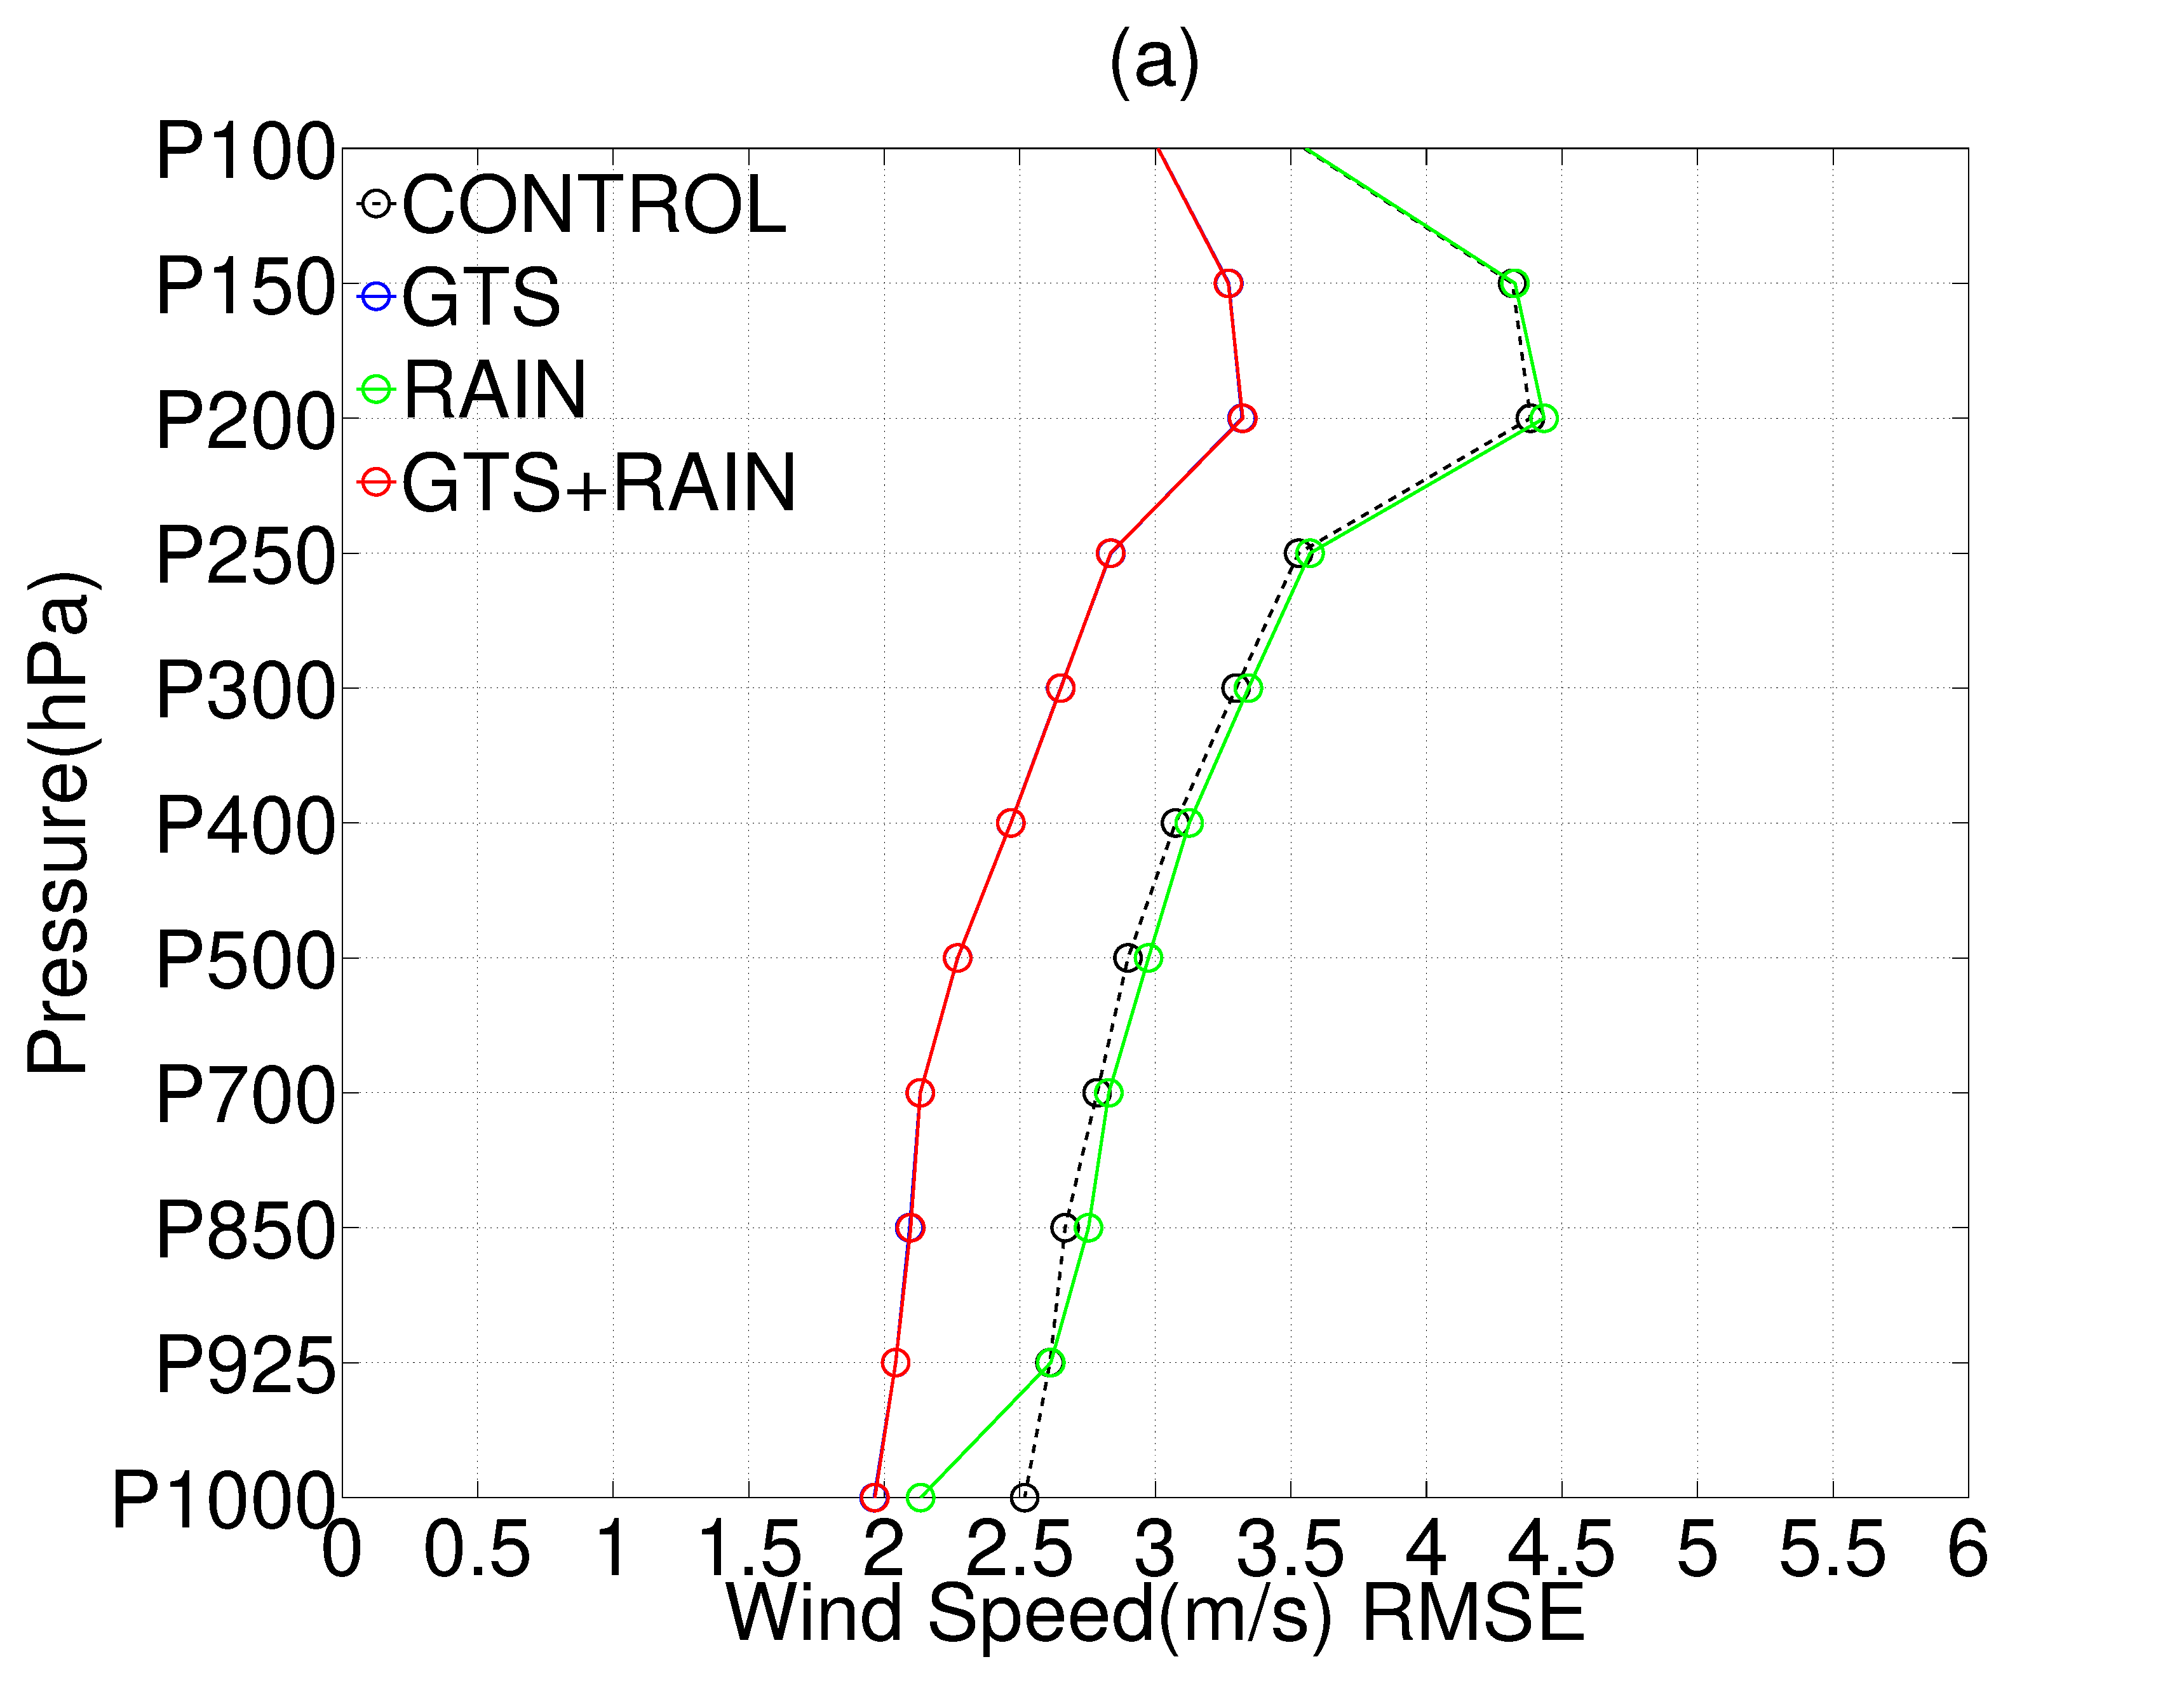
\includegraphics[width=19pc,angle=0]{wind_00.eps}\\
  \noindent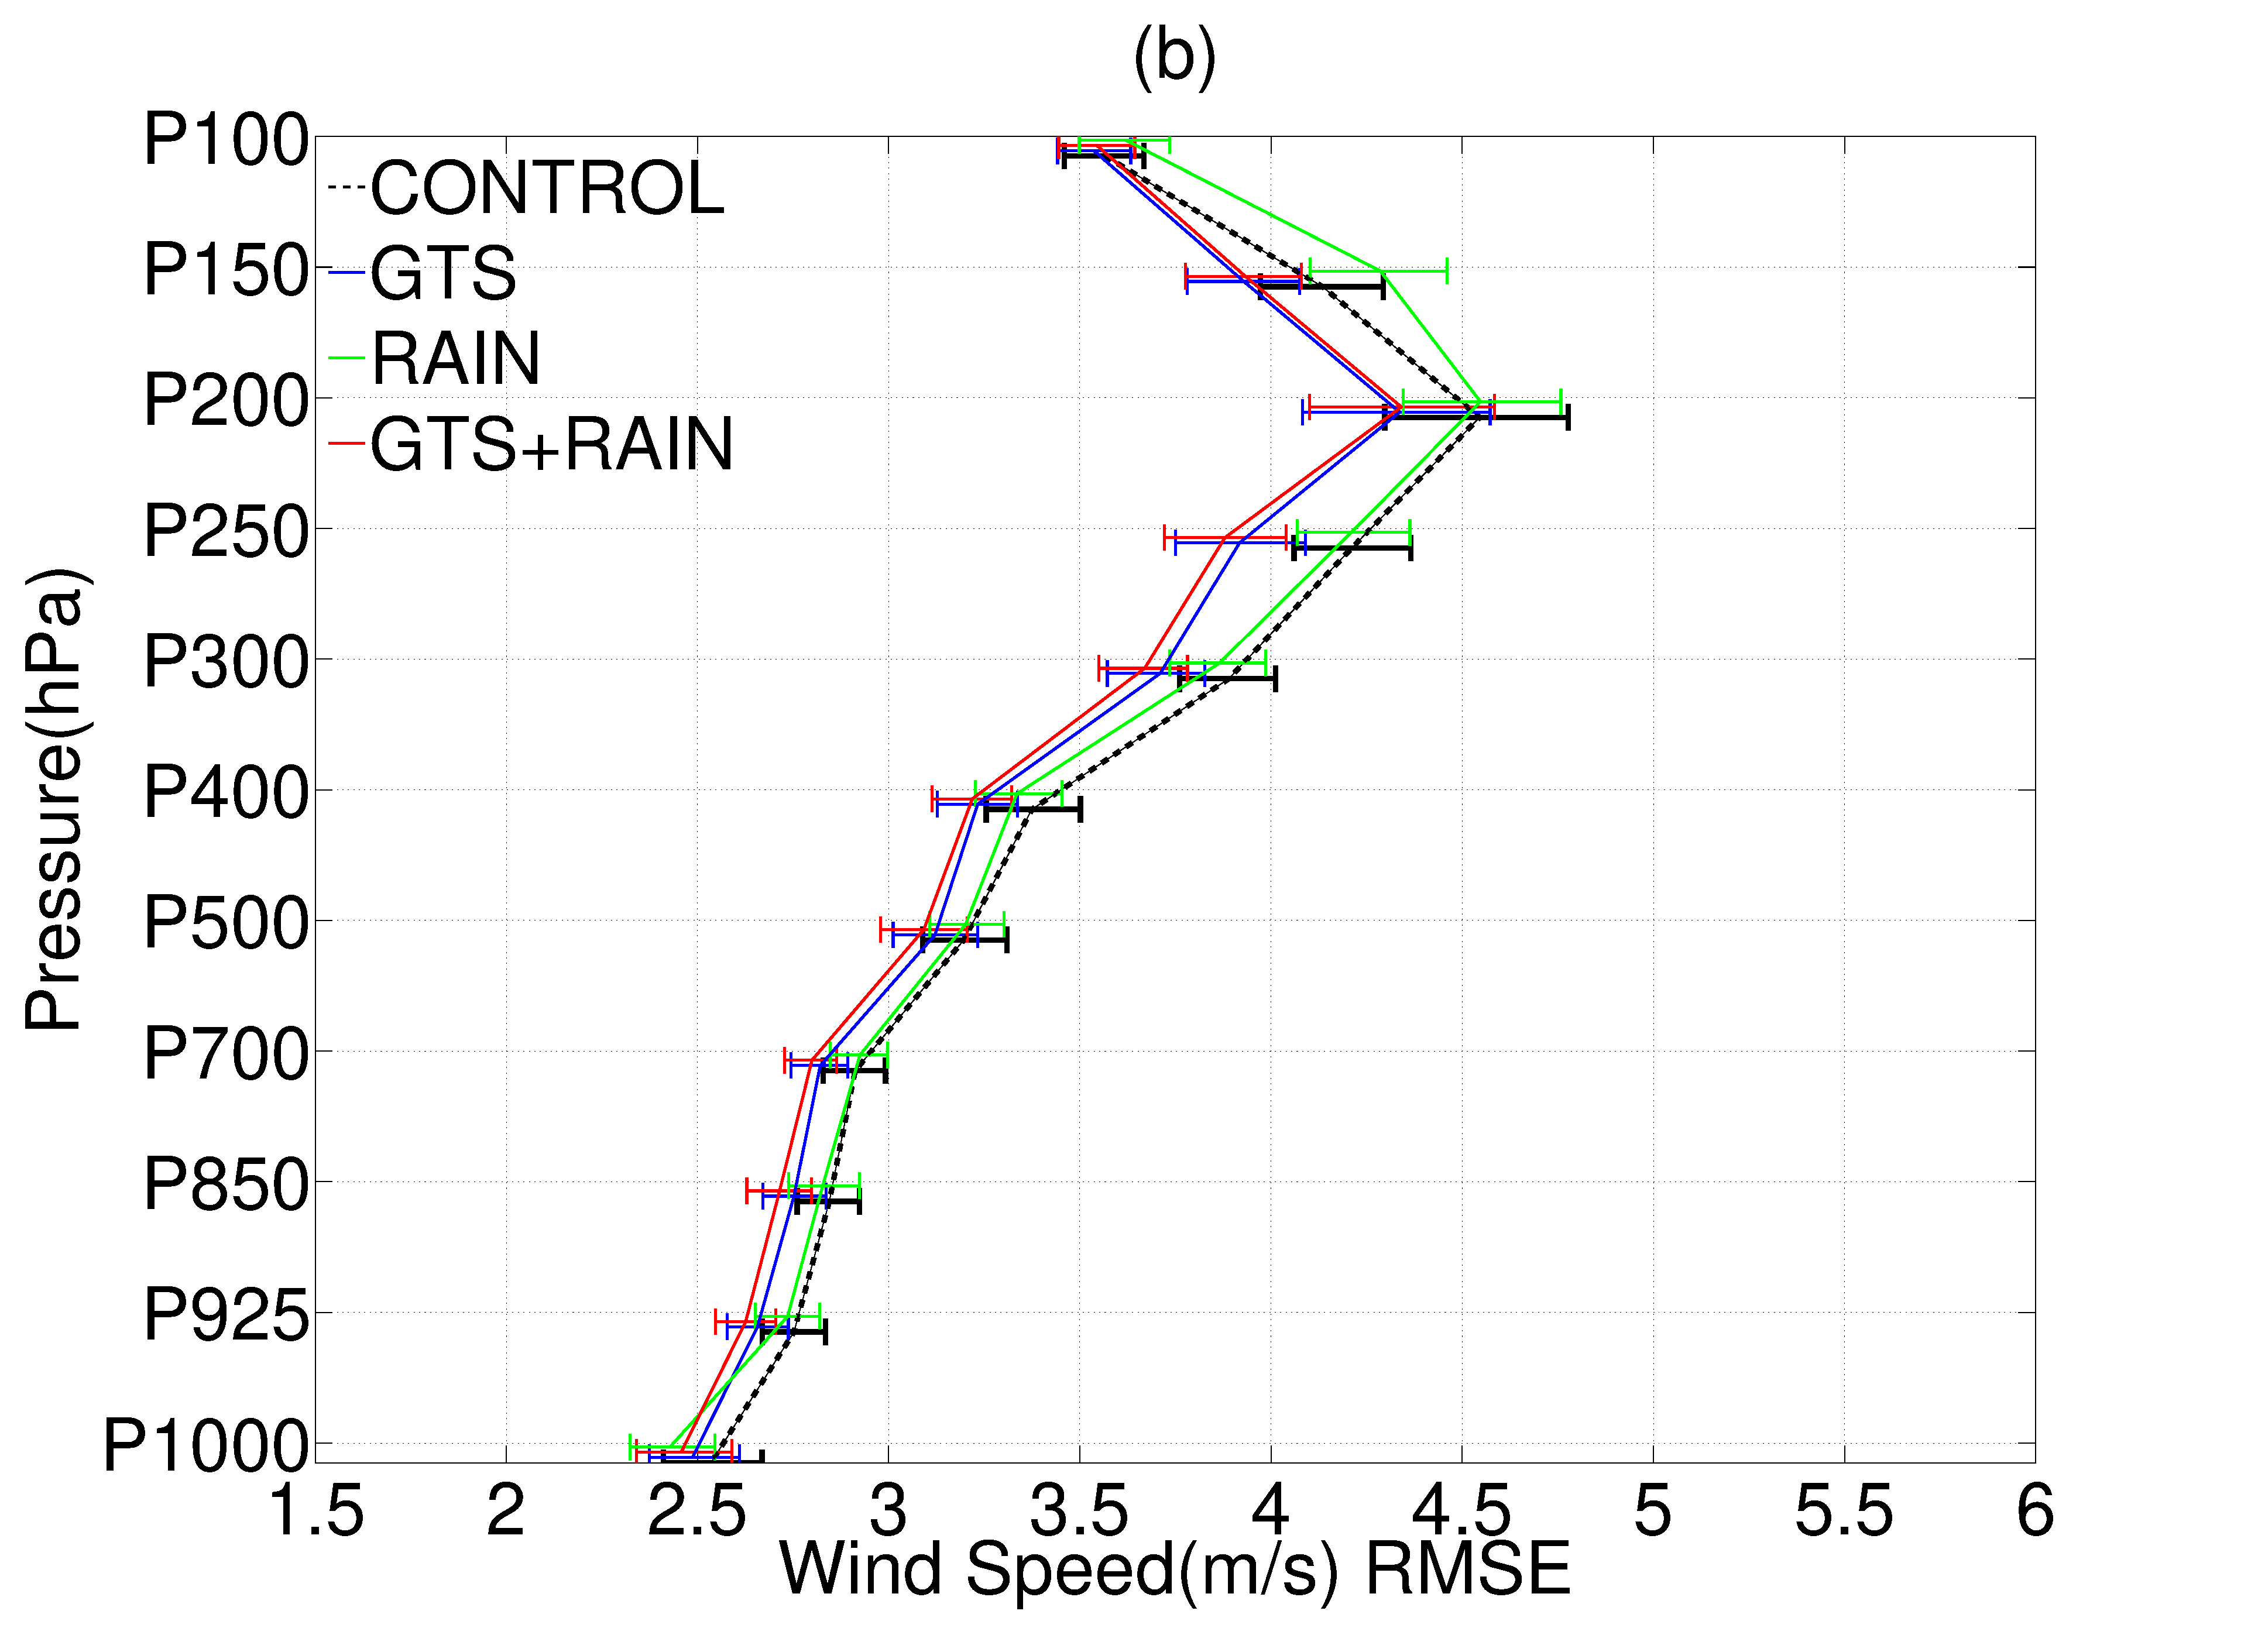
\includegraphics[width=19pc,angle=0]{wind_12.eps}\\
  \noindent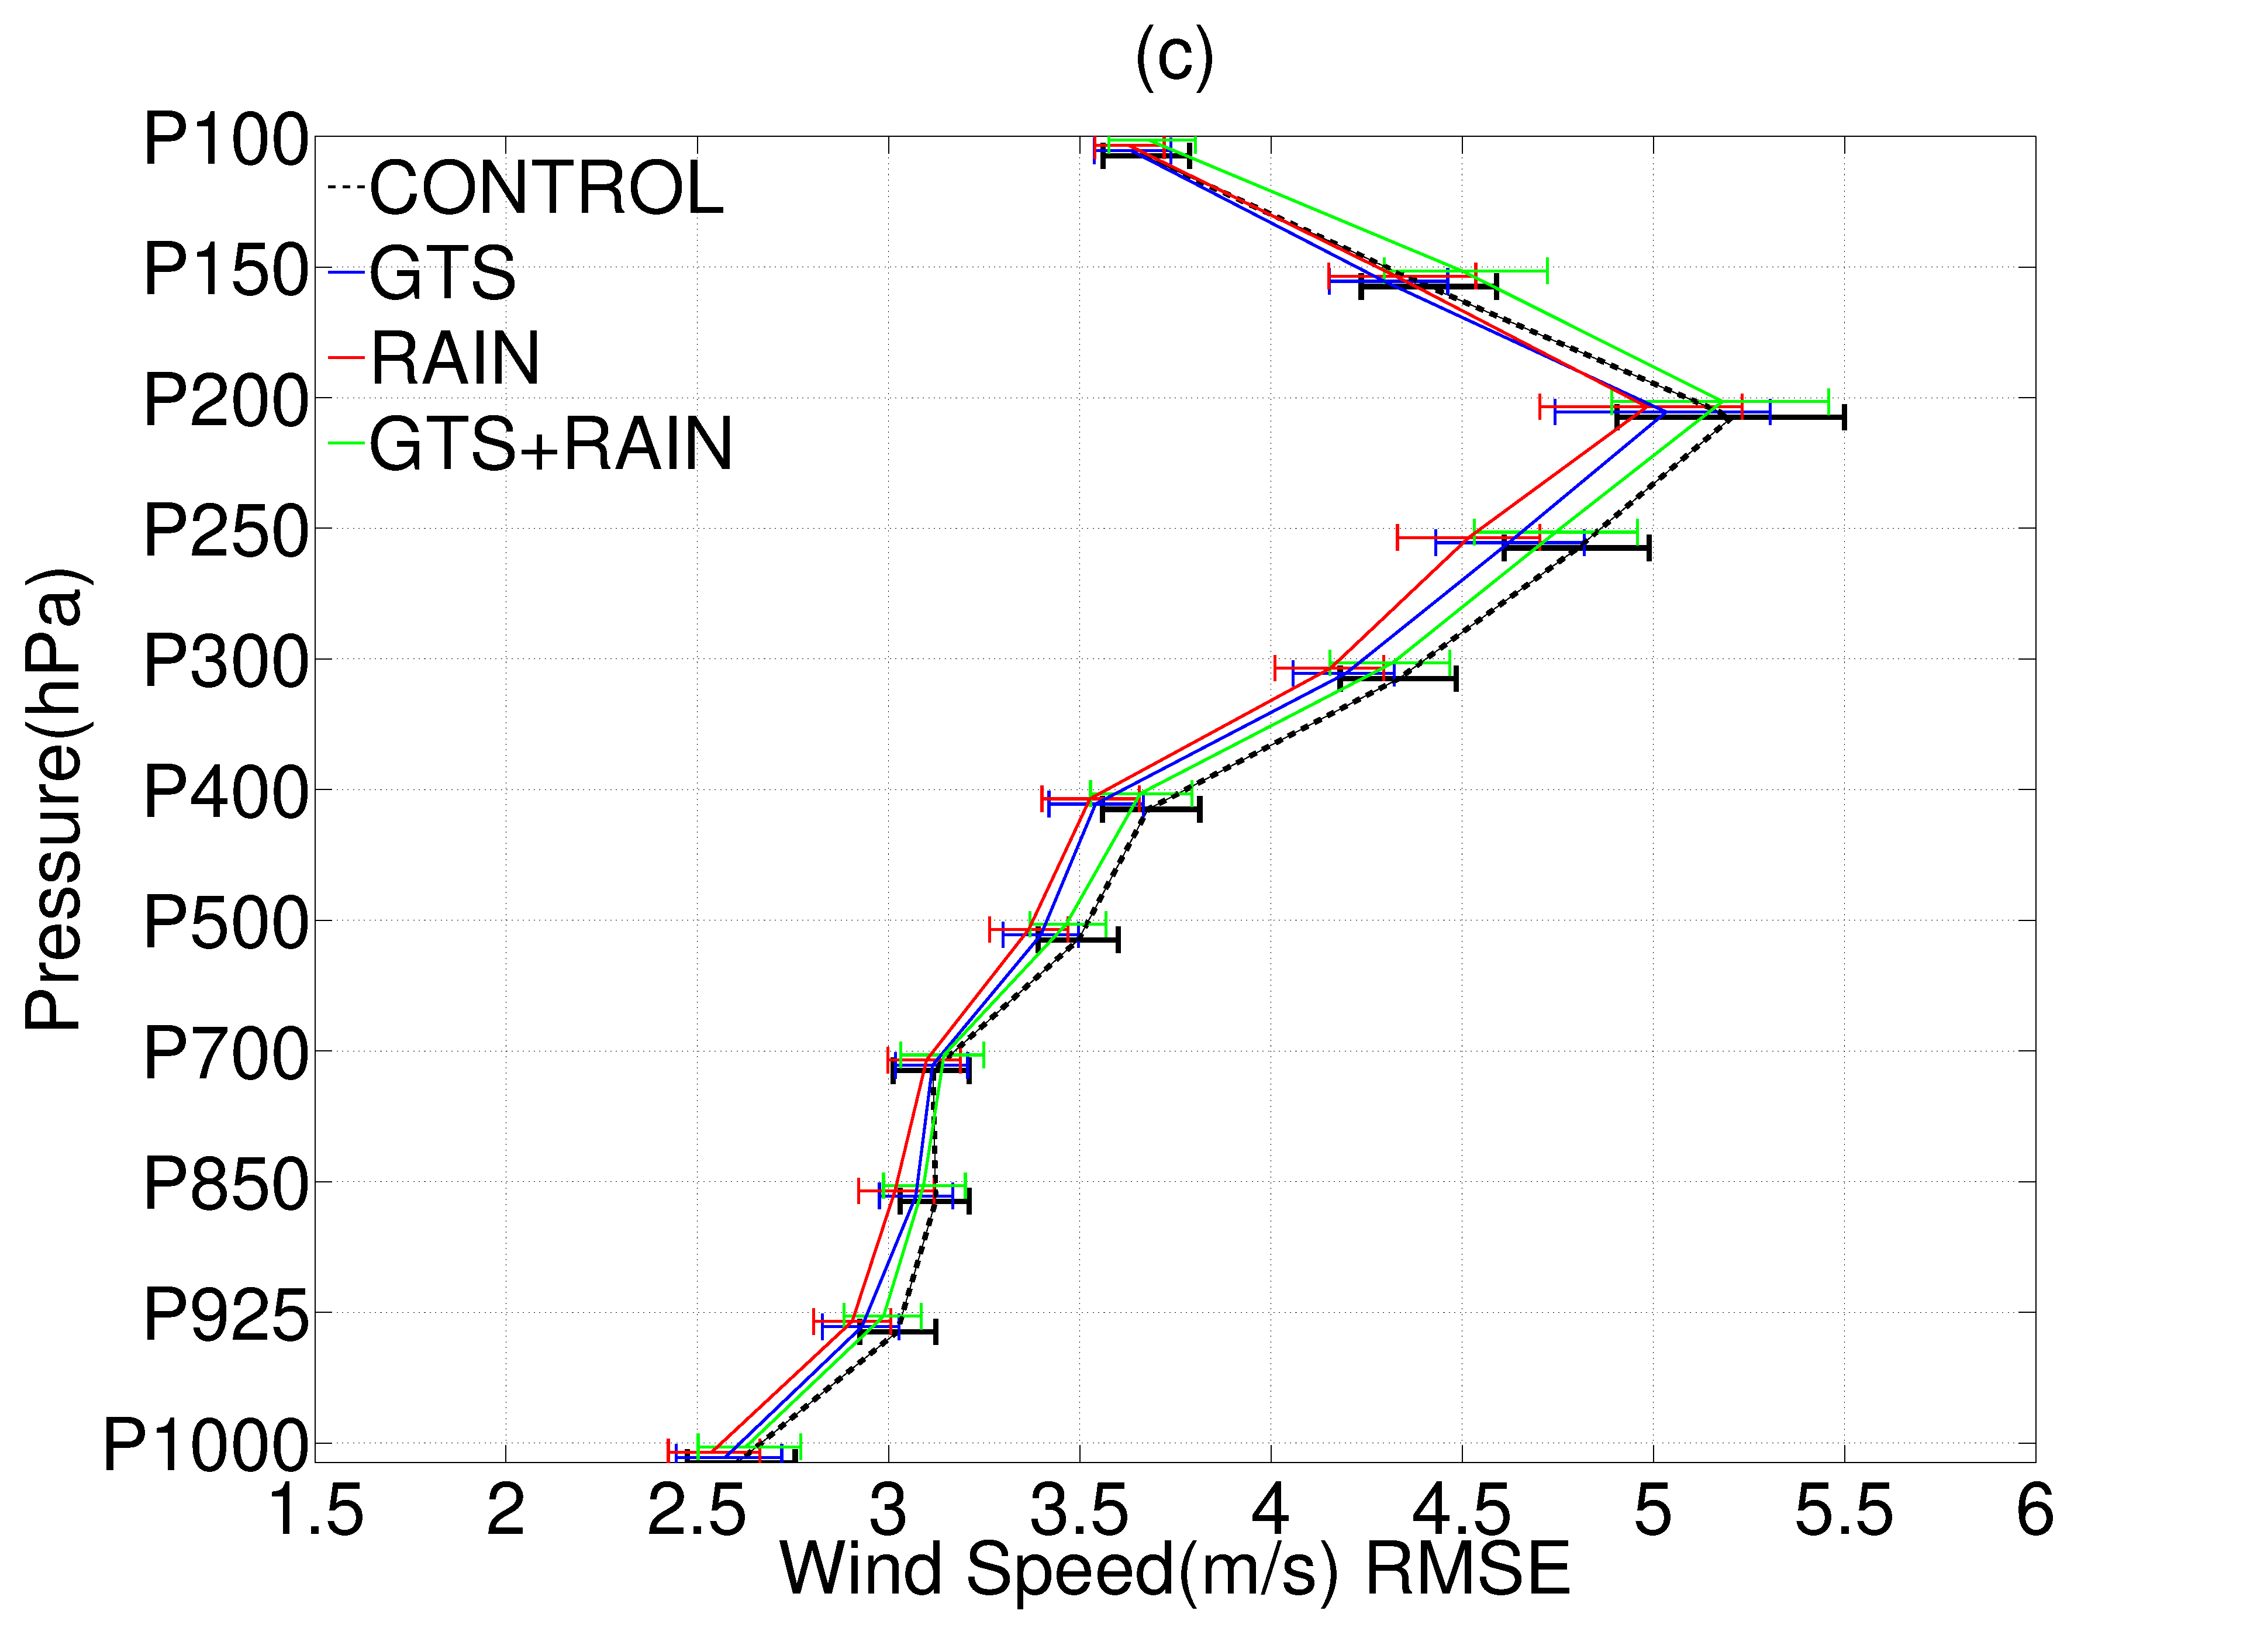
\includegraphics[width=19pc,angle=0]{wind_24.eps}\\  
  \caption{Vertical profiles of the RMSEs of wind speed for experiments CONTROL, GTS, RAIN and GTS+RAIN for analysis (a), 12-h forecast(b) and 24-h forecast(c) aggregated over 1-month period of the case verified against upper air sounding data. The horizontal bars represent the confidence intervals at the 95\% confidence level. }  
\label{f1}  
\end{figure}

\begin{figure}
  \noindent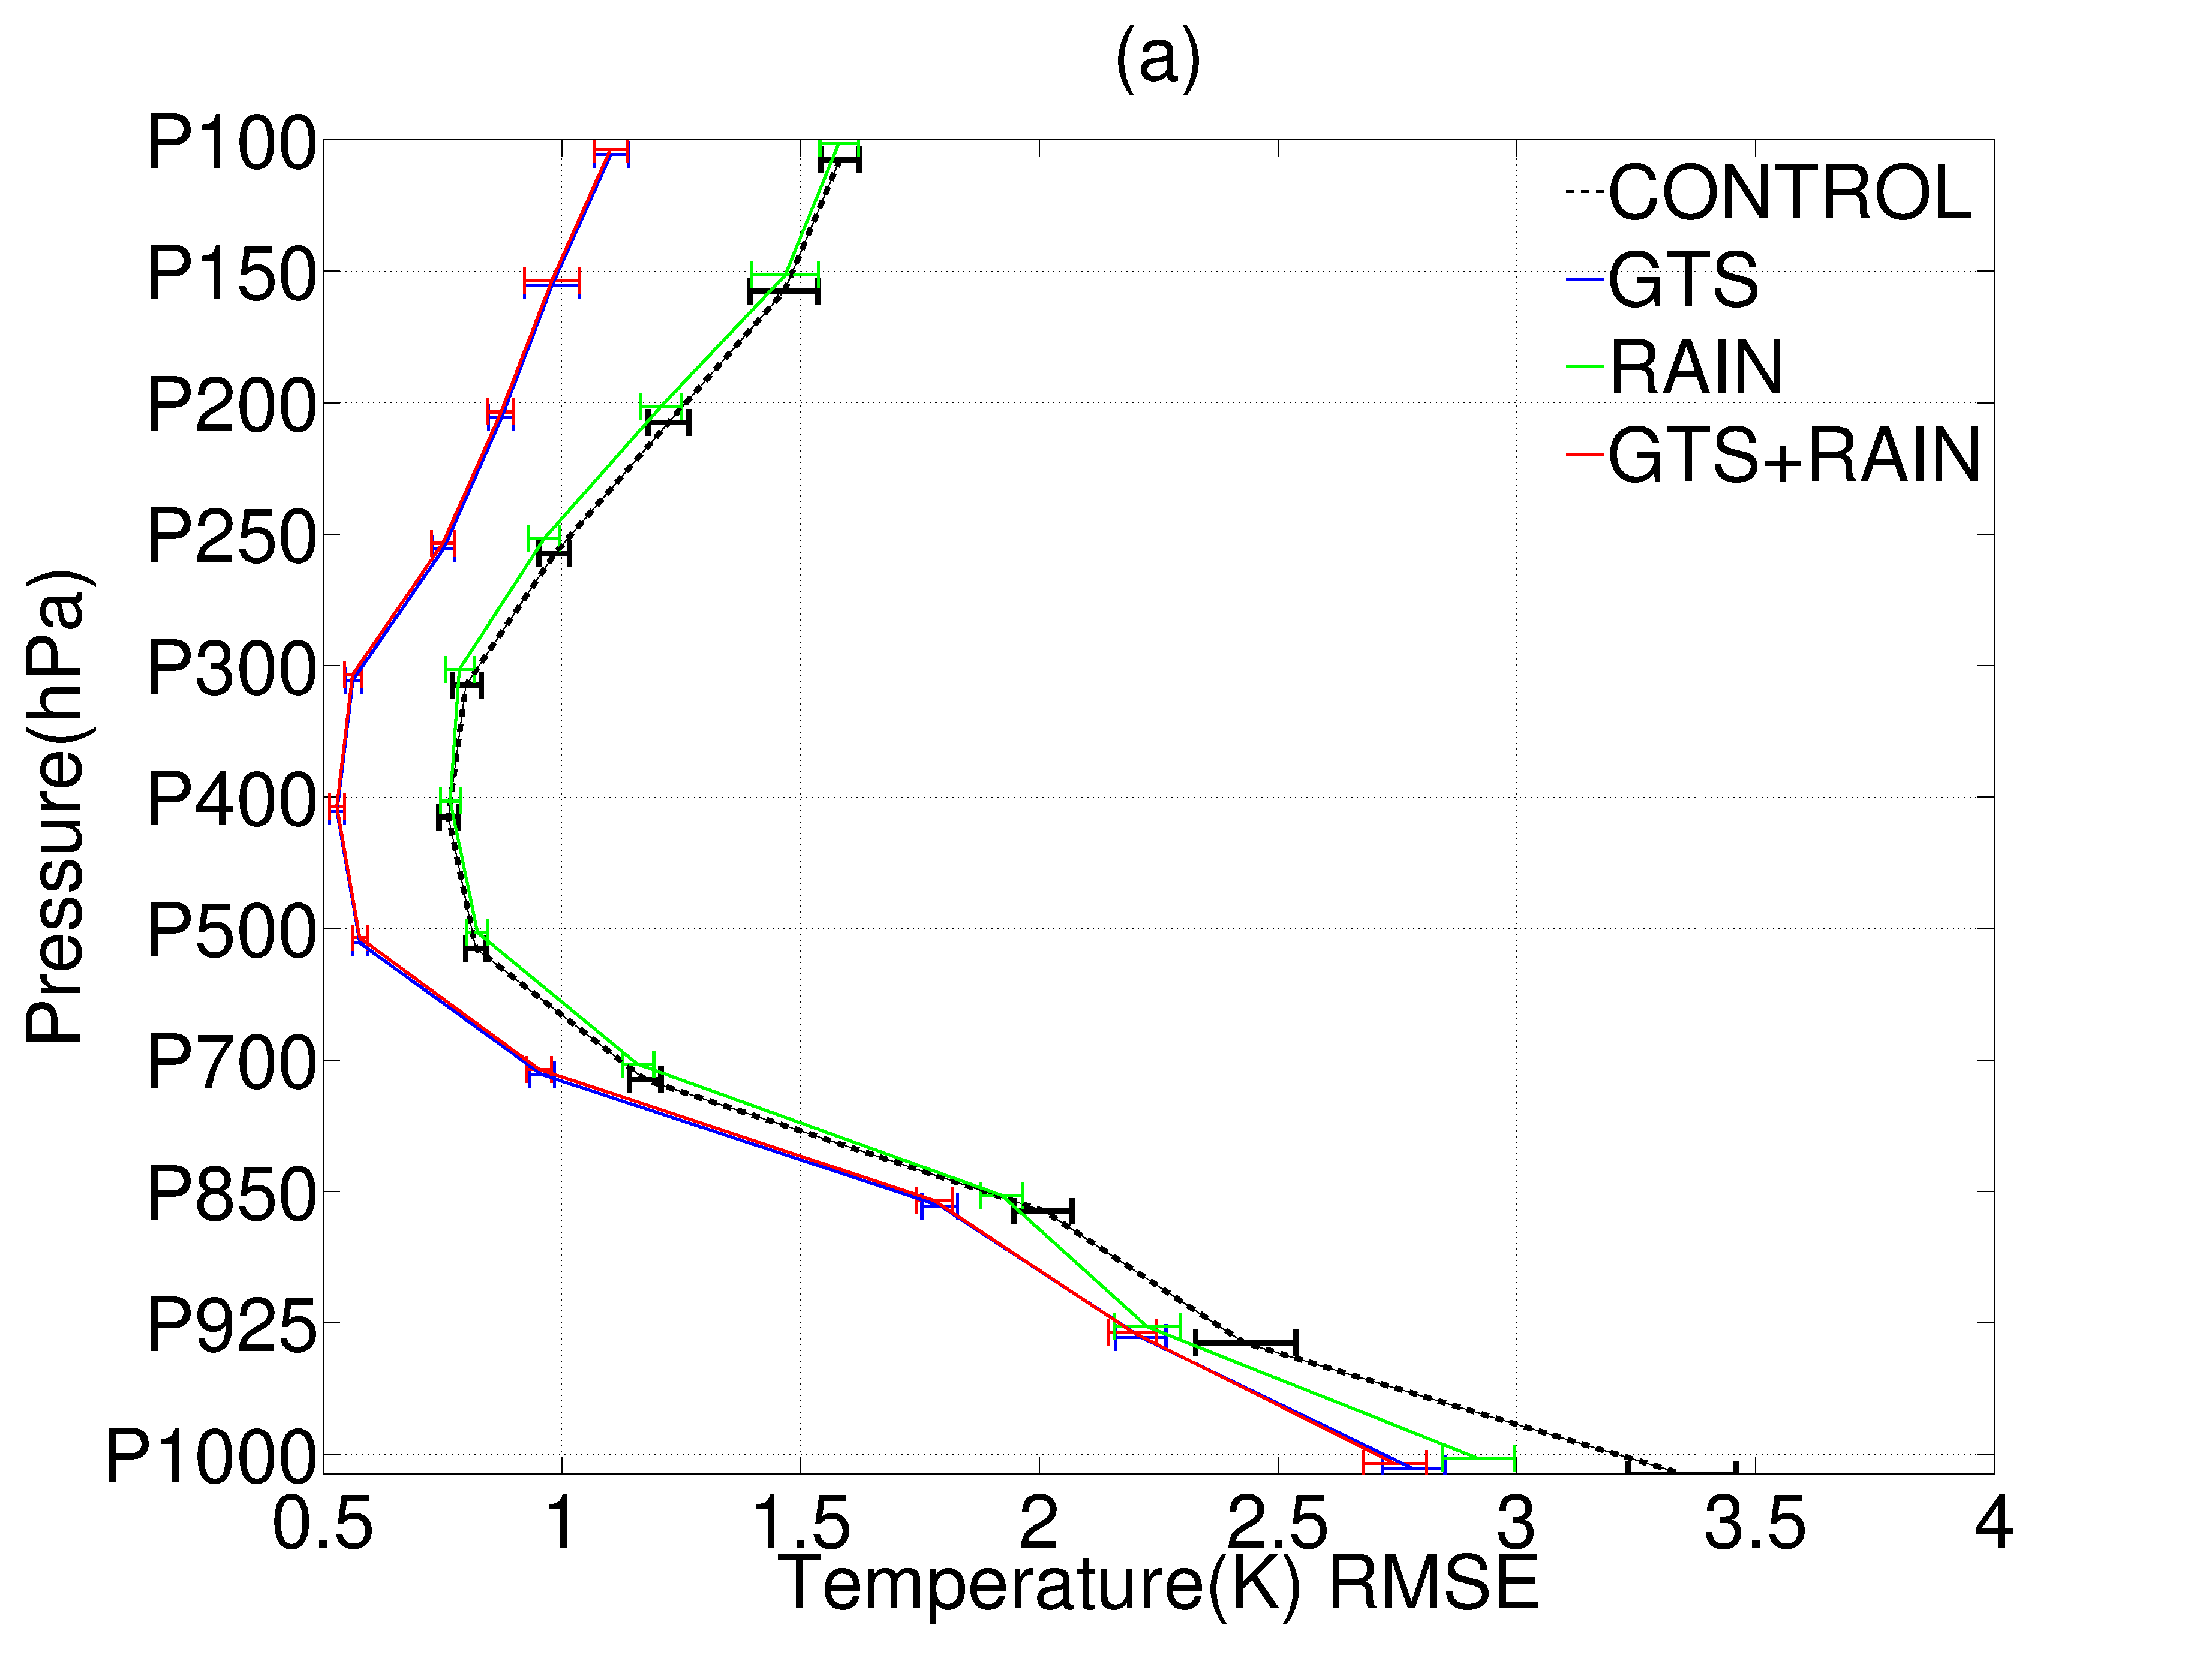
\includegraphics[width=19pc,angle=0]{tmp_00.eps}\\
  \noindent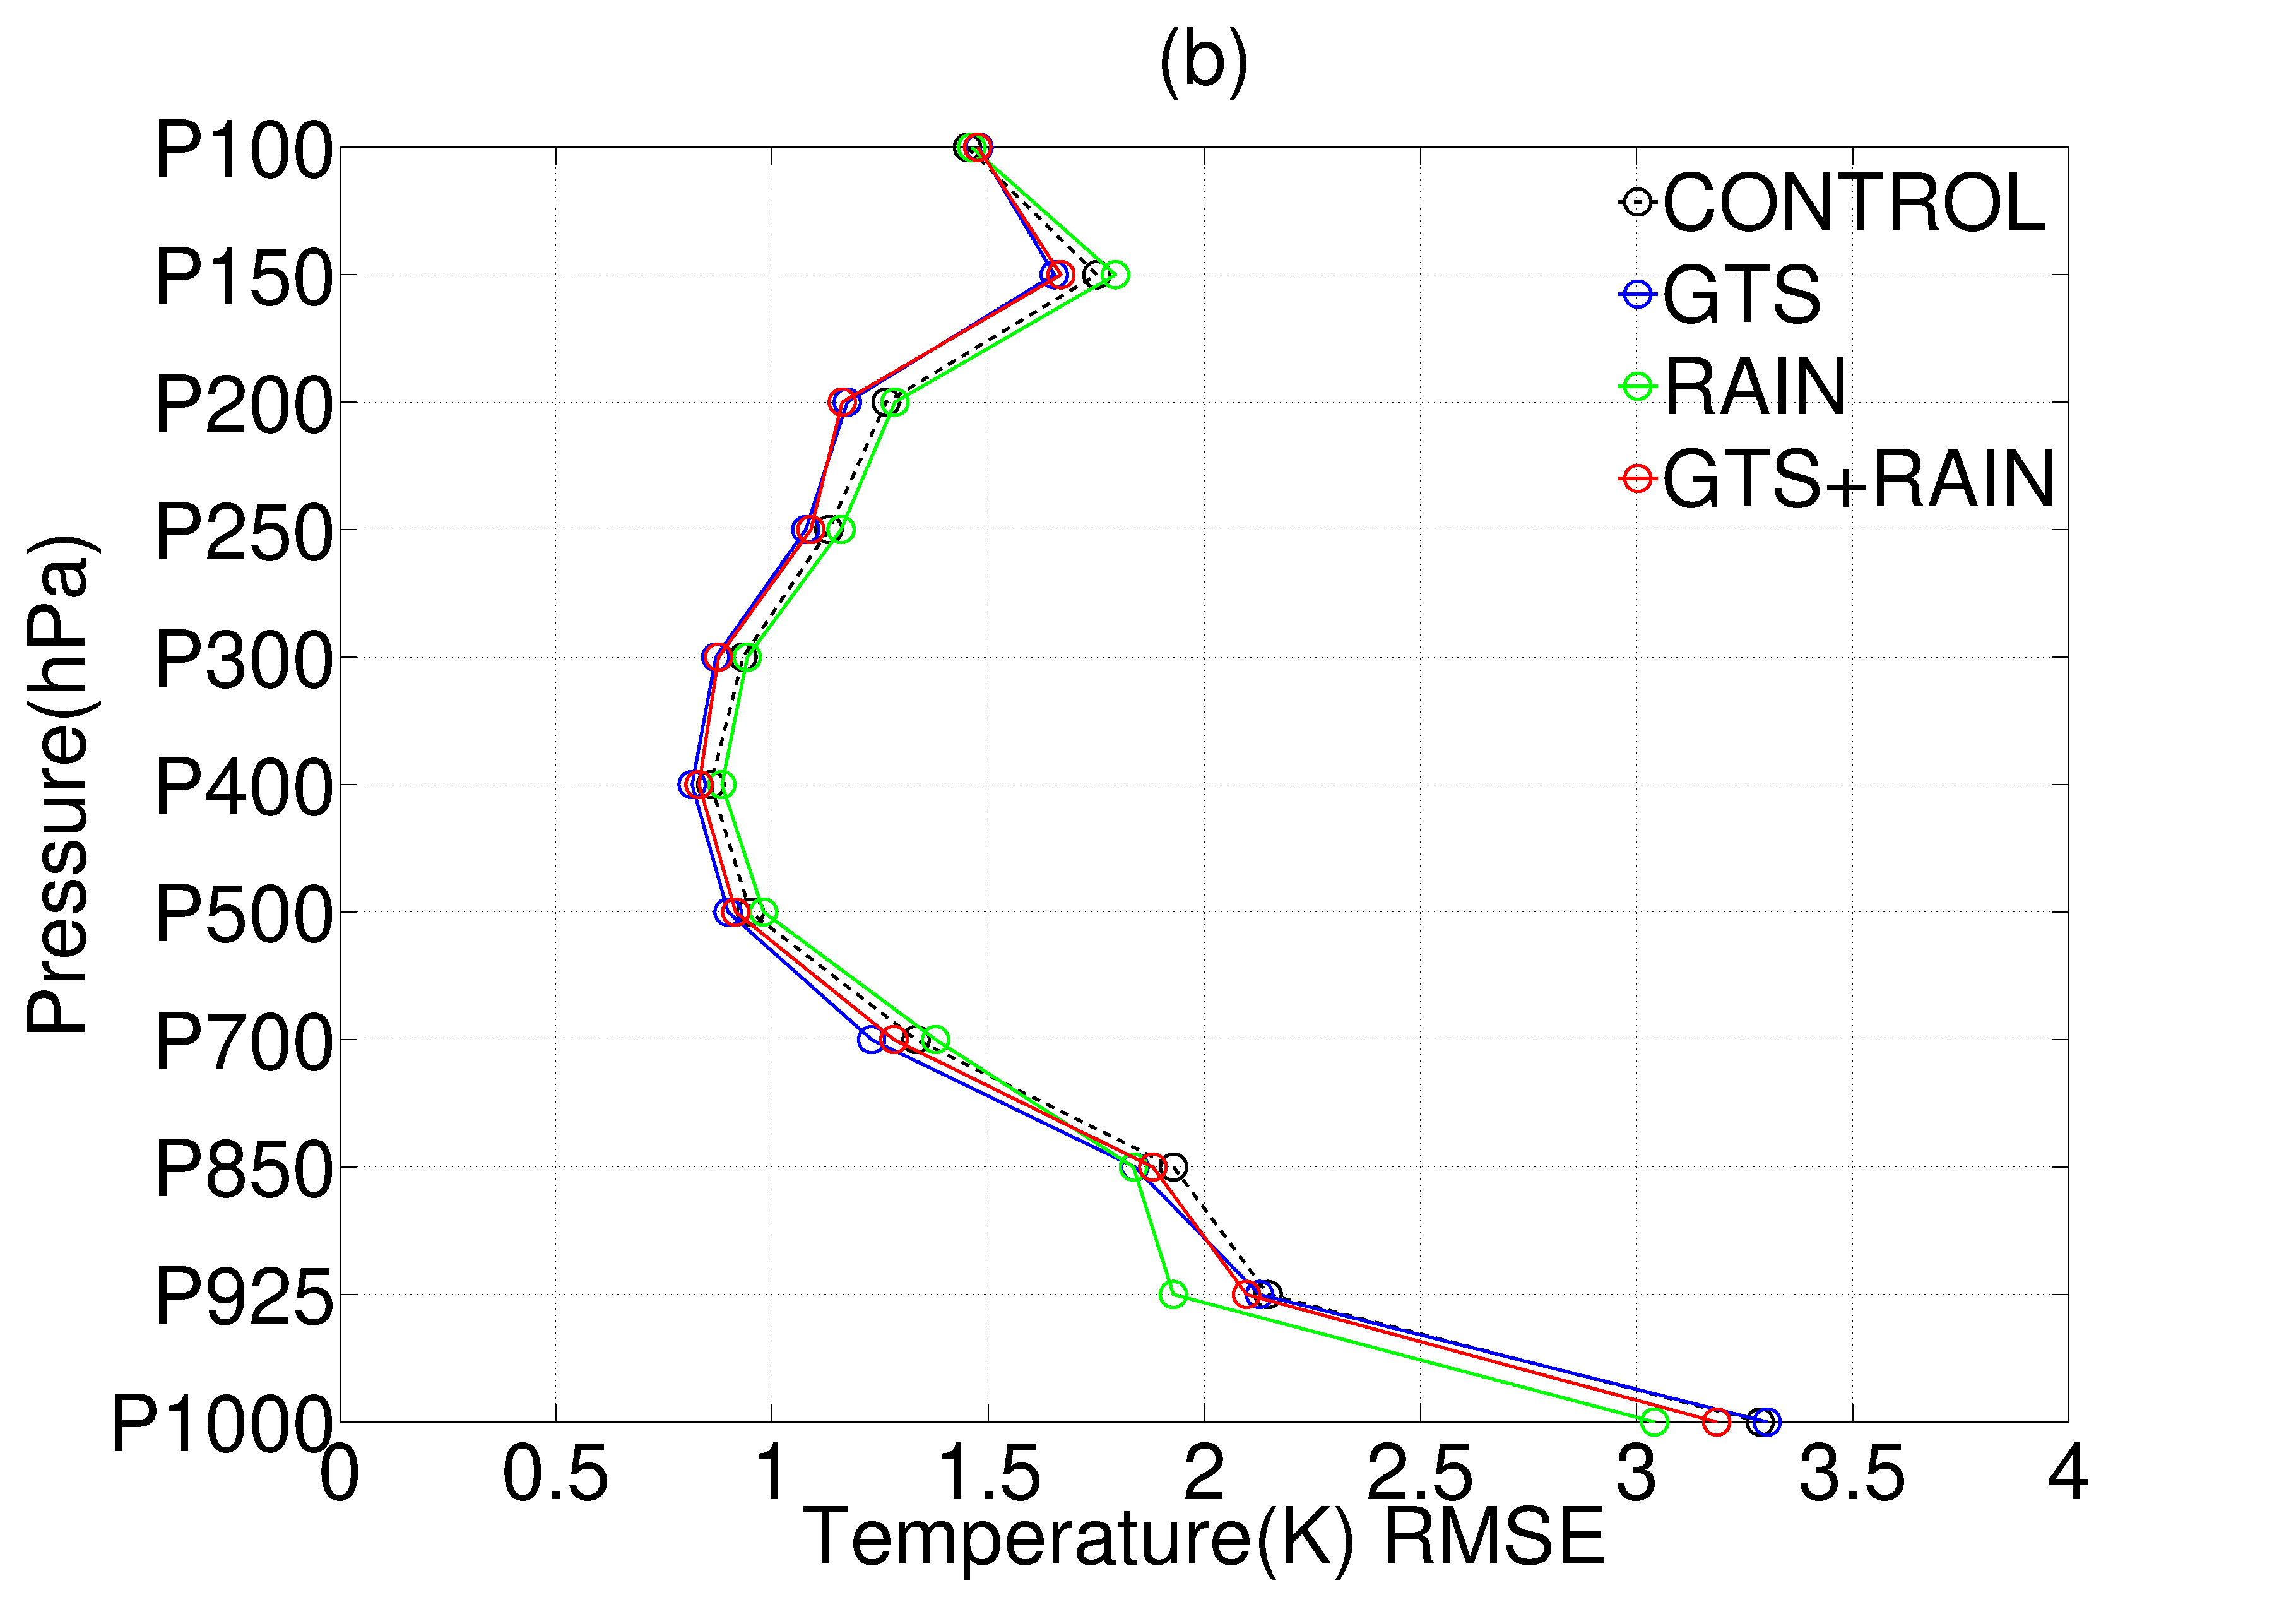
\includegraphics[width=19pc,angle=0]{tmp_12.eps}\\
  \noindent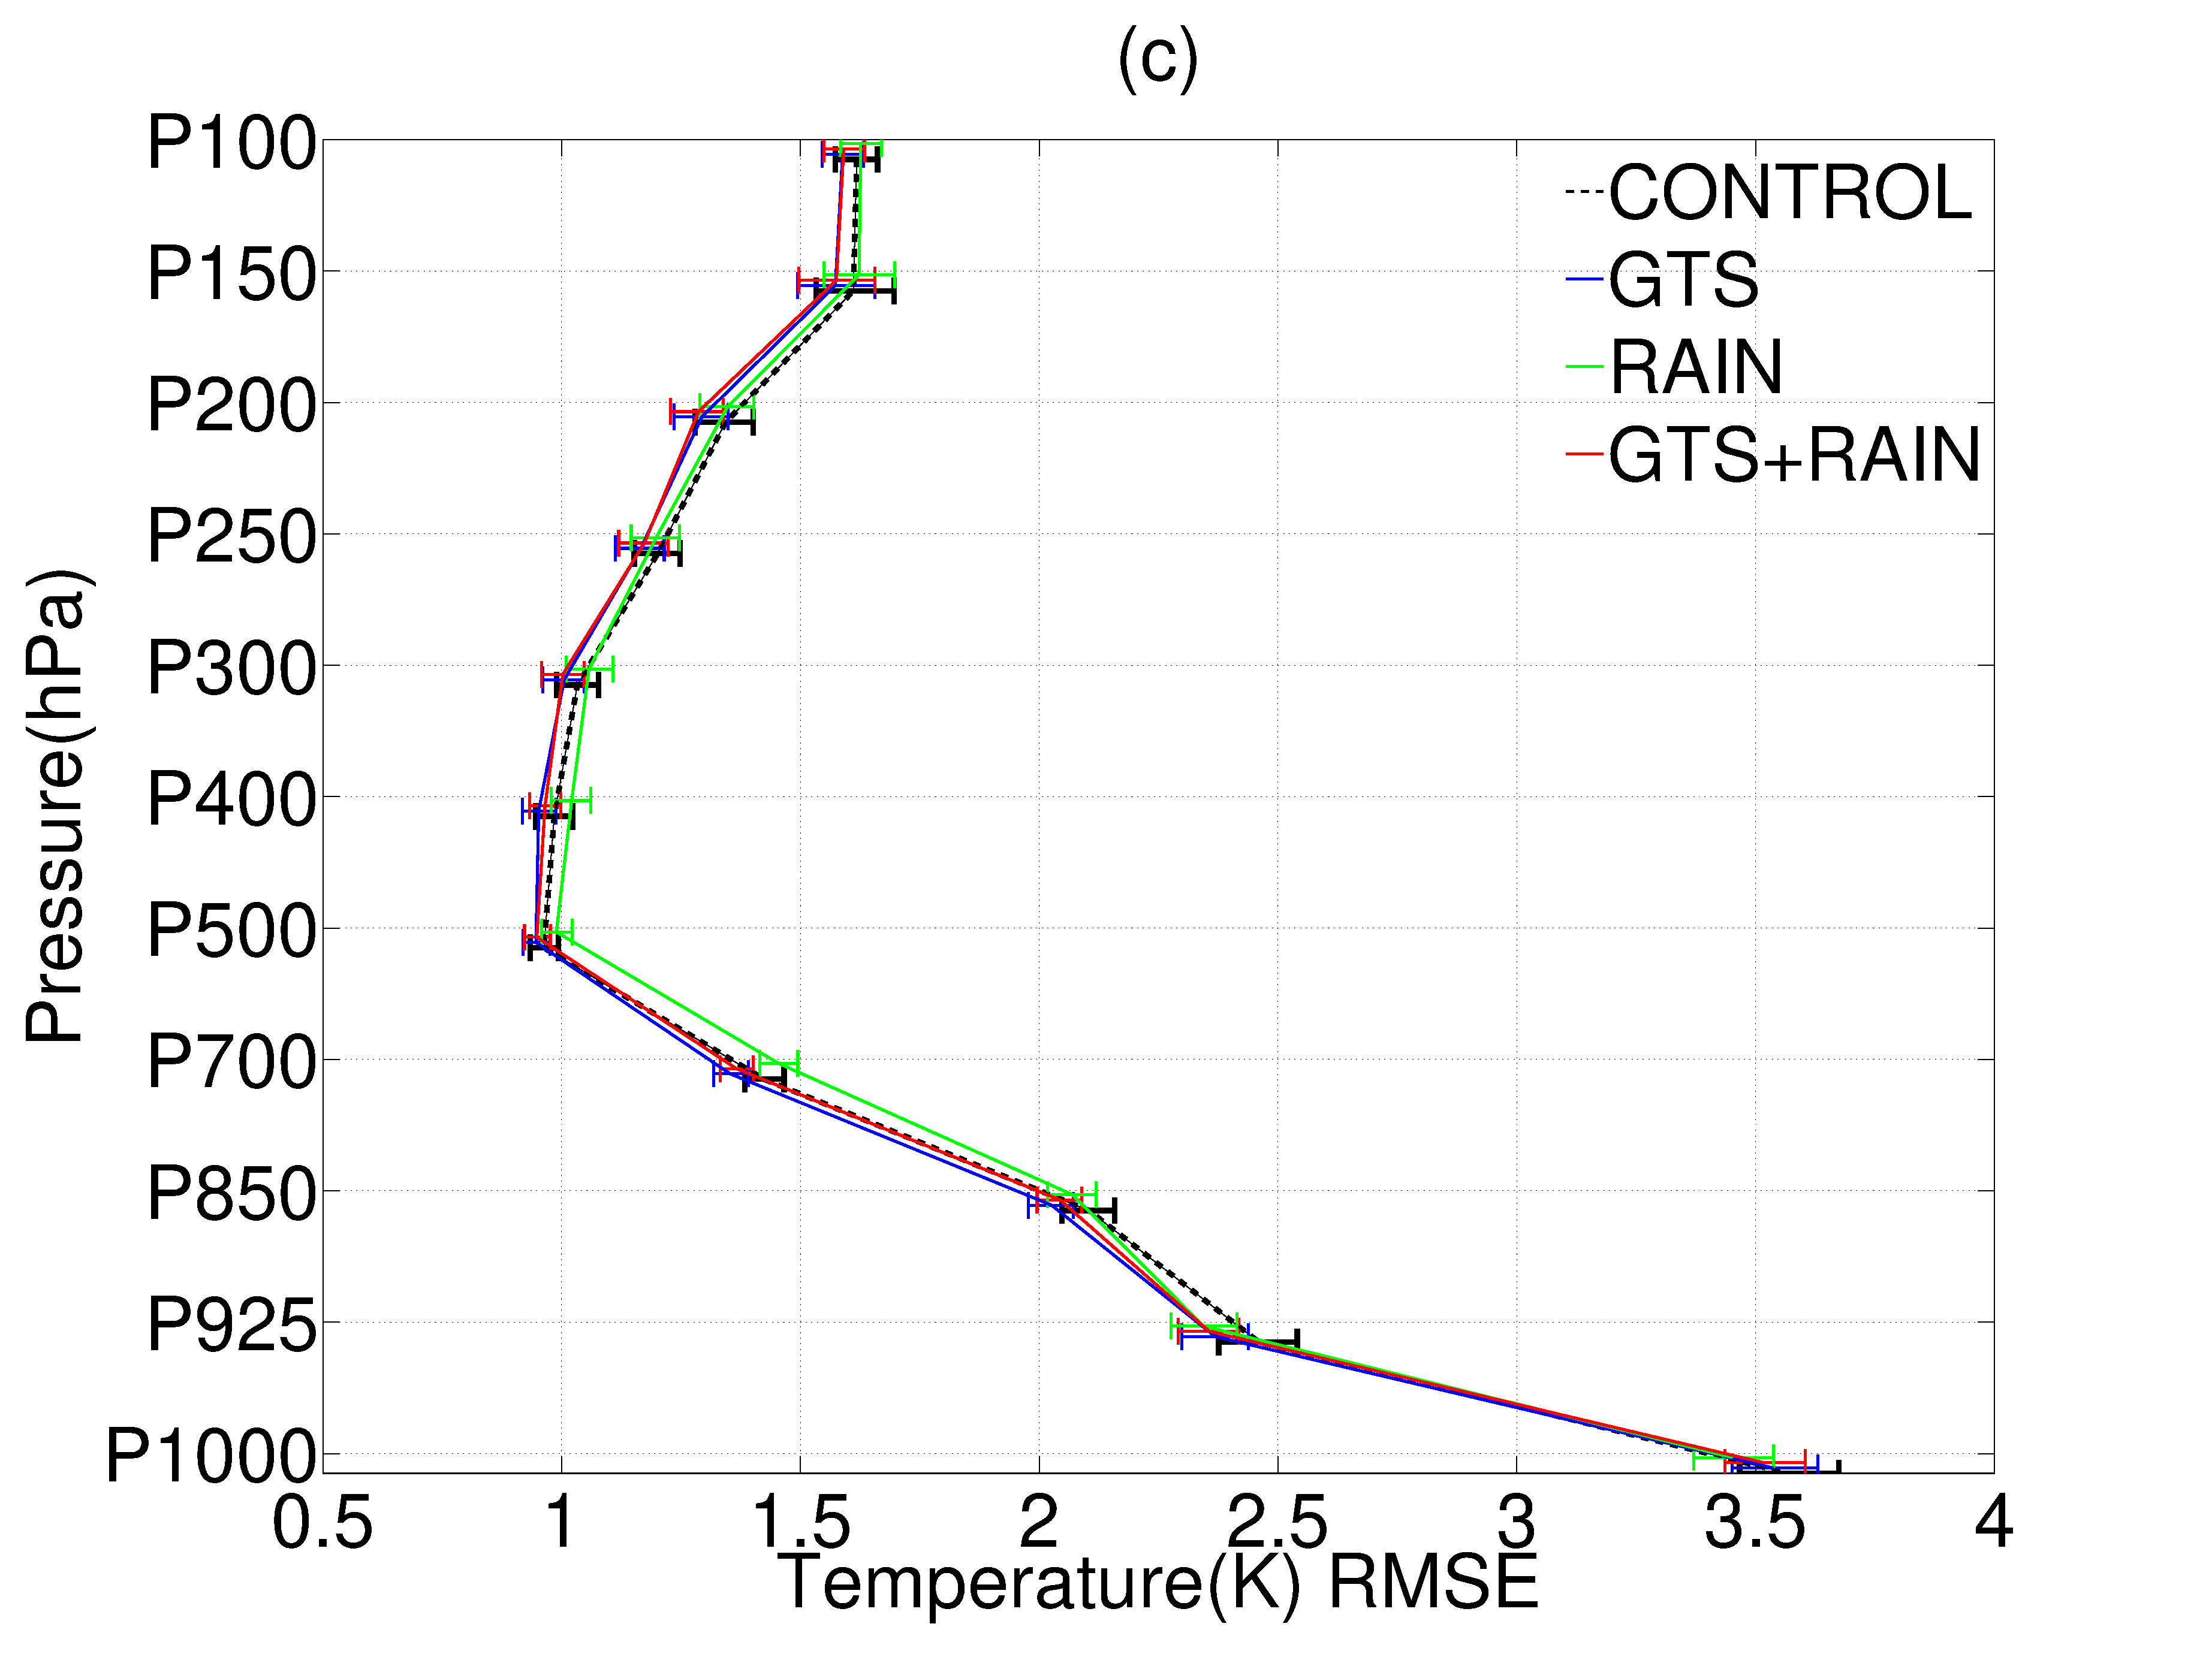
\includegraphics[width=19pc,angle=0]{tmp_24.eps}\\  
   \caption{Same as Figure 1 but for temperature.}
   \label{f2}
\end{figure}

\begin{figure}
  \noindent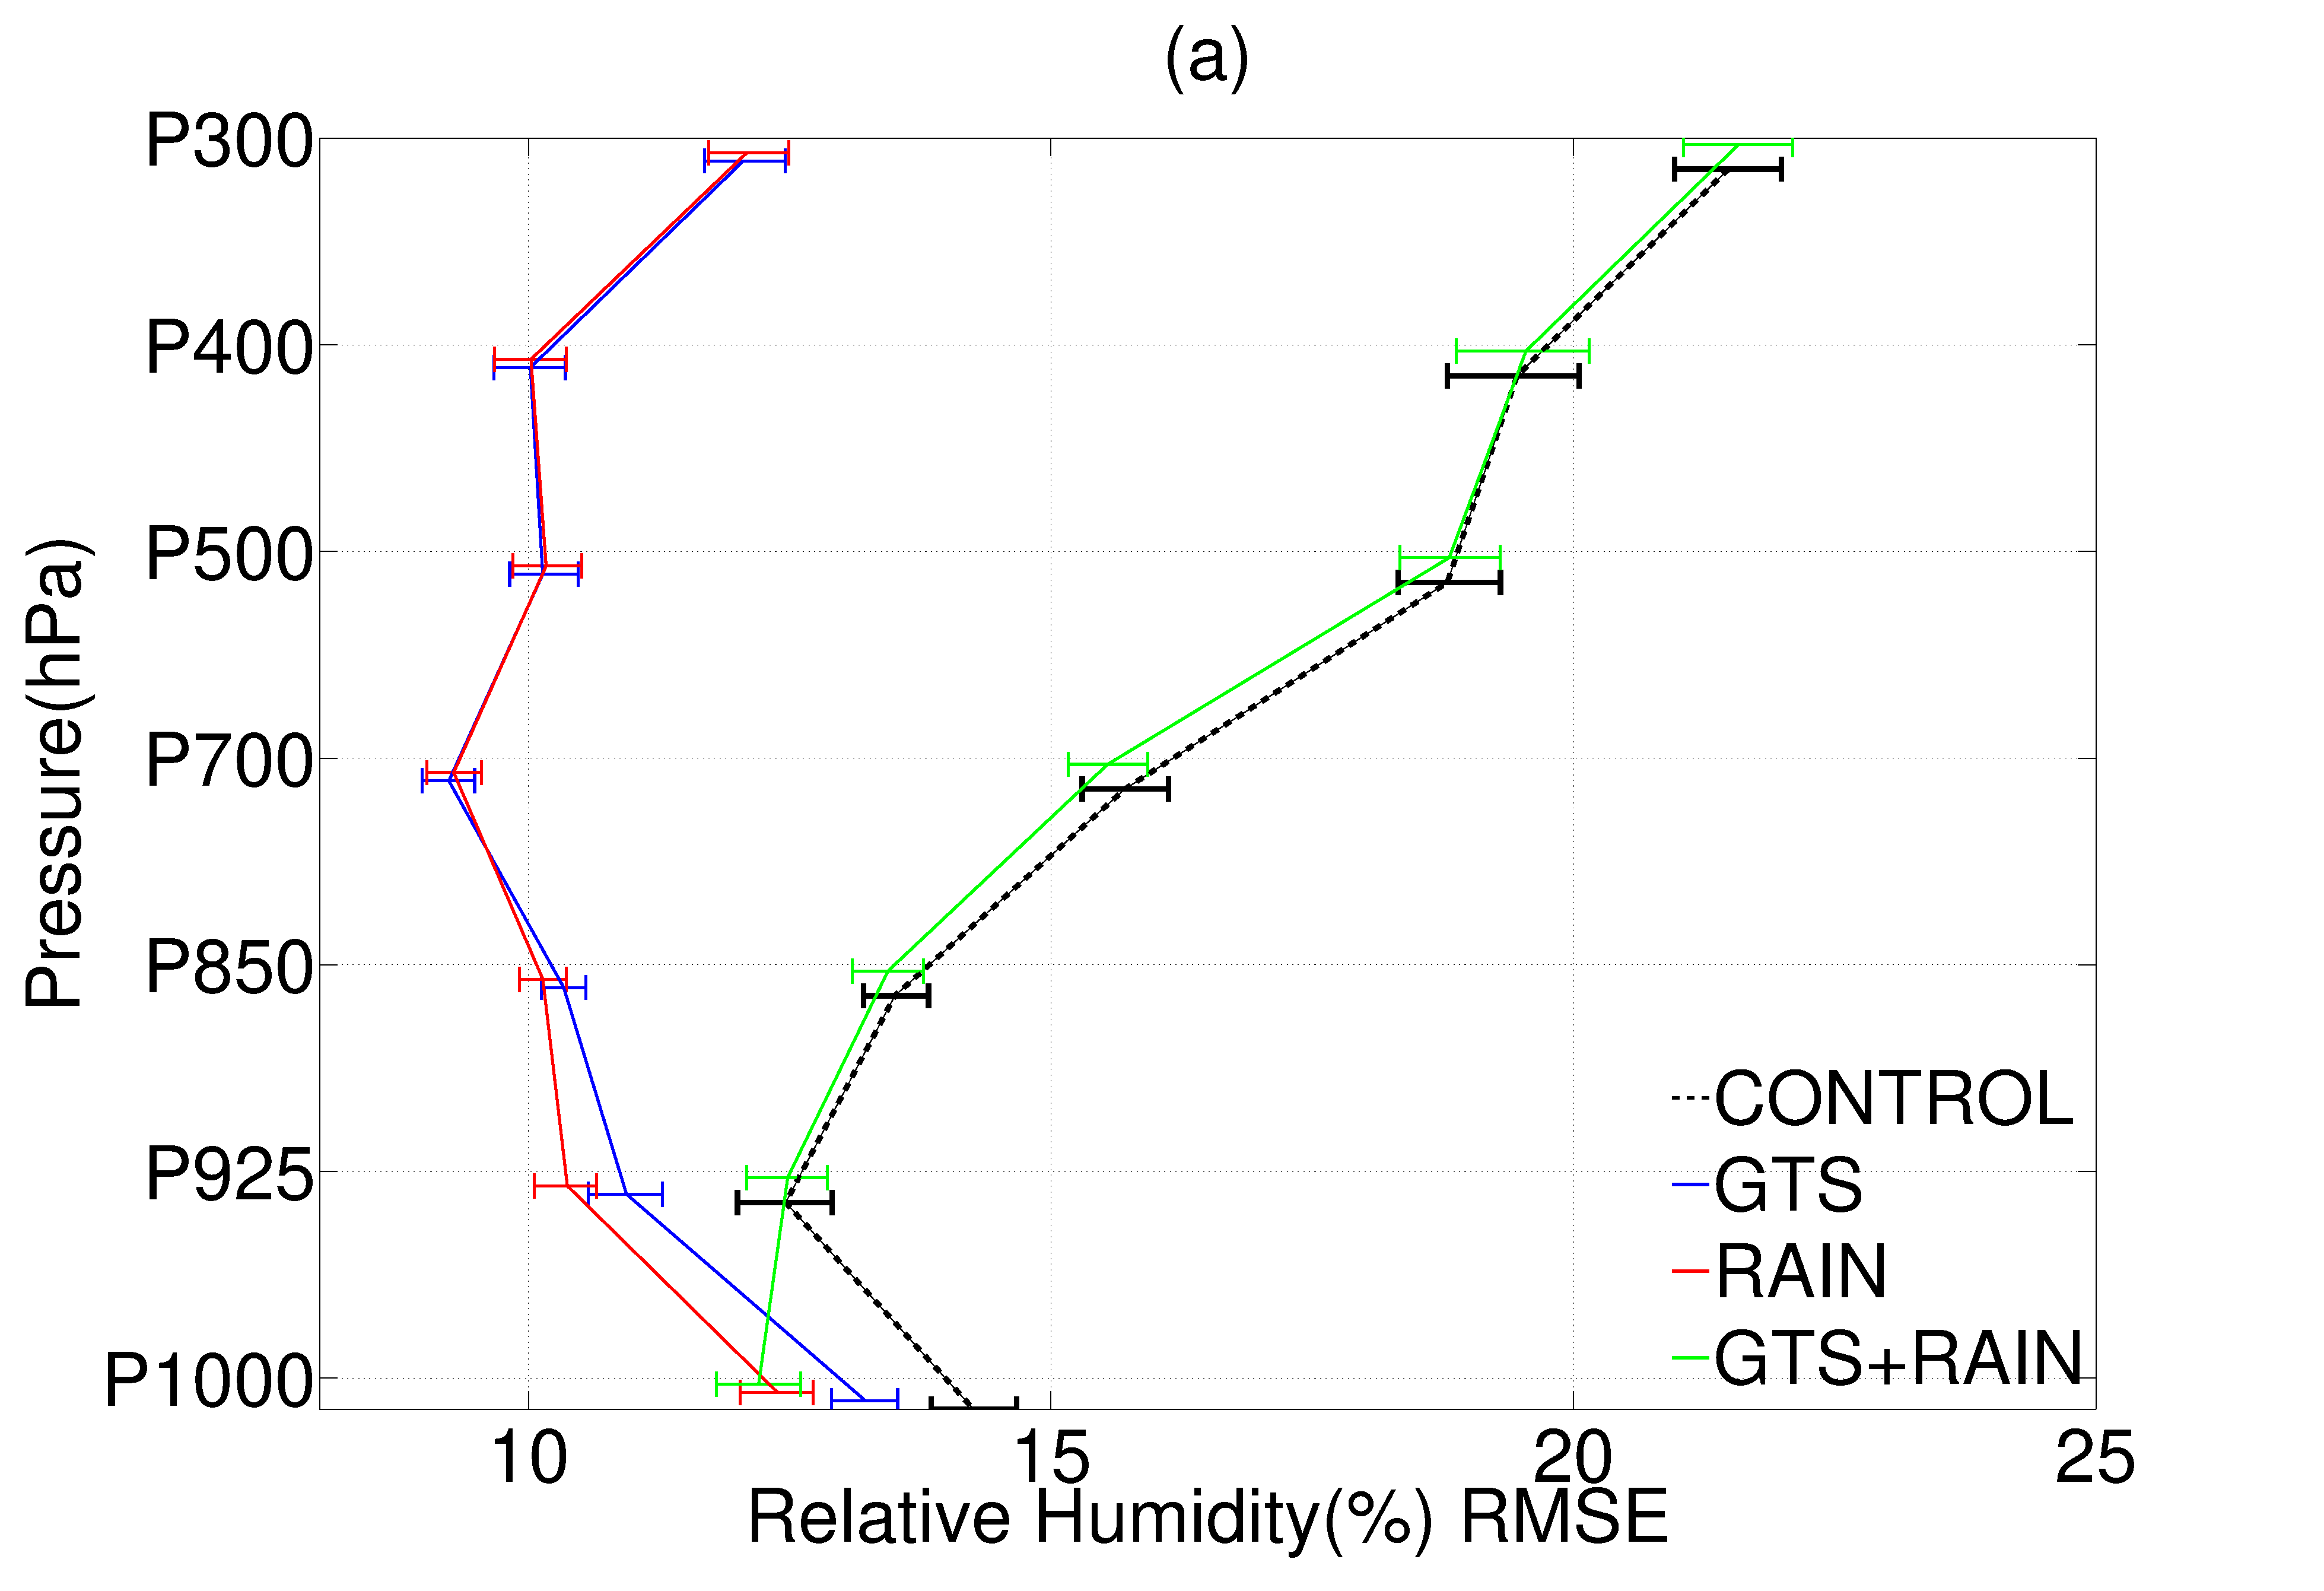
\includegraphics[width=19pc,angle=0]{rh_00.eps}\\
  \noindent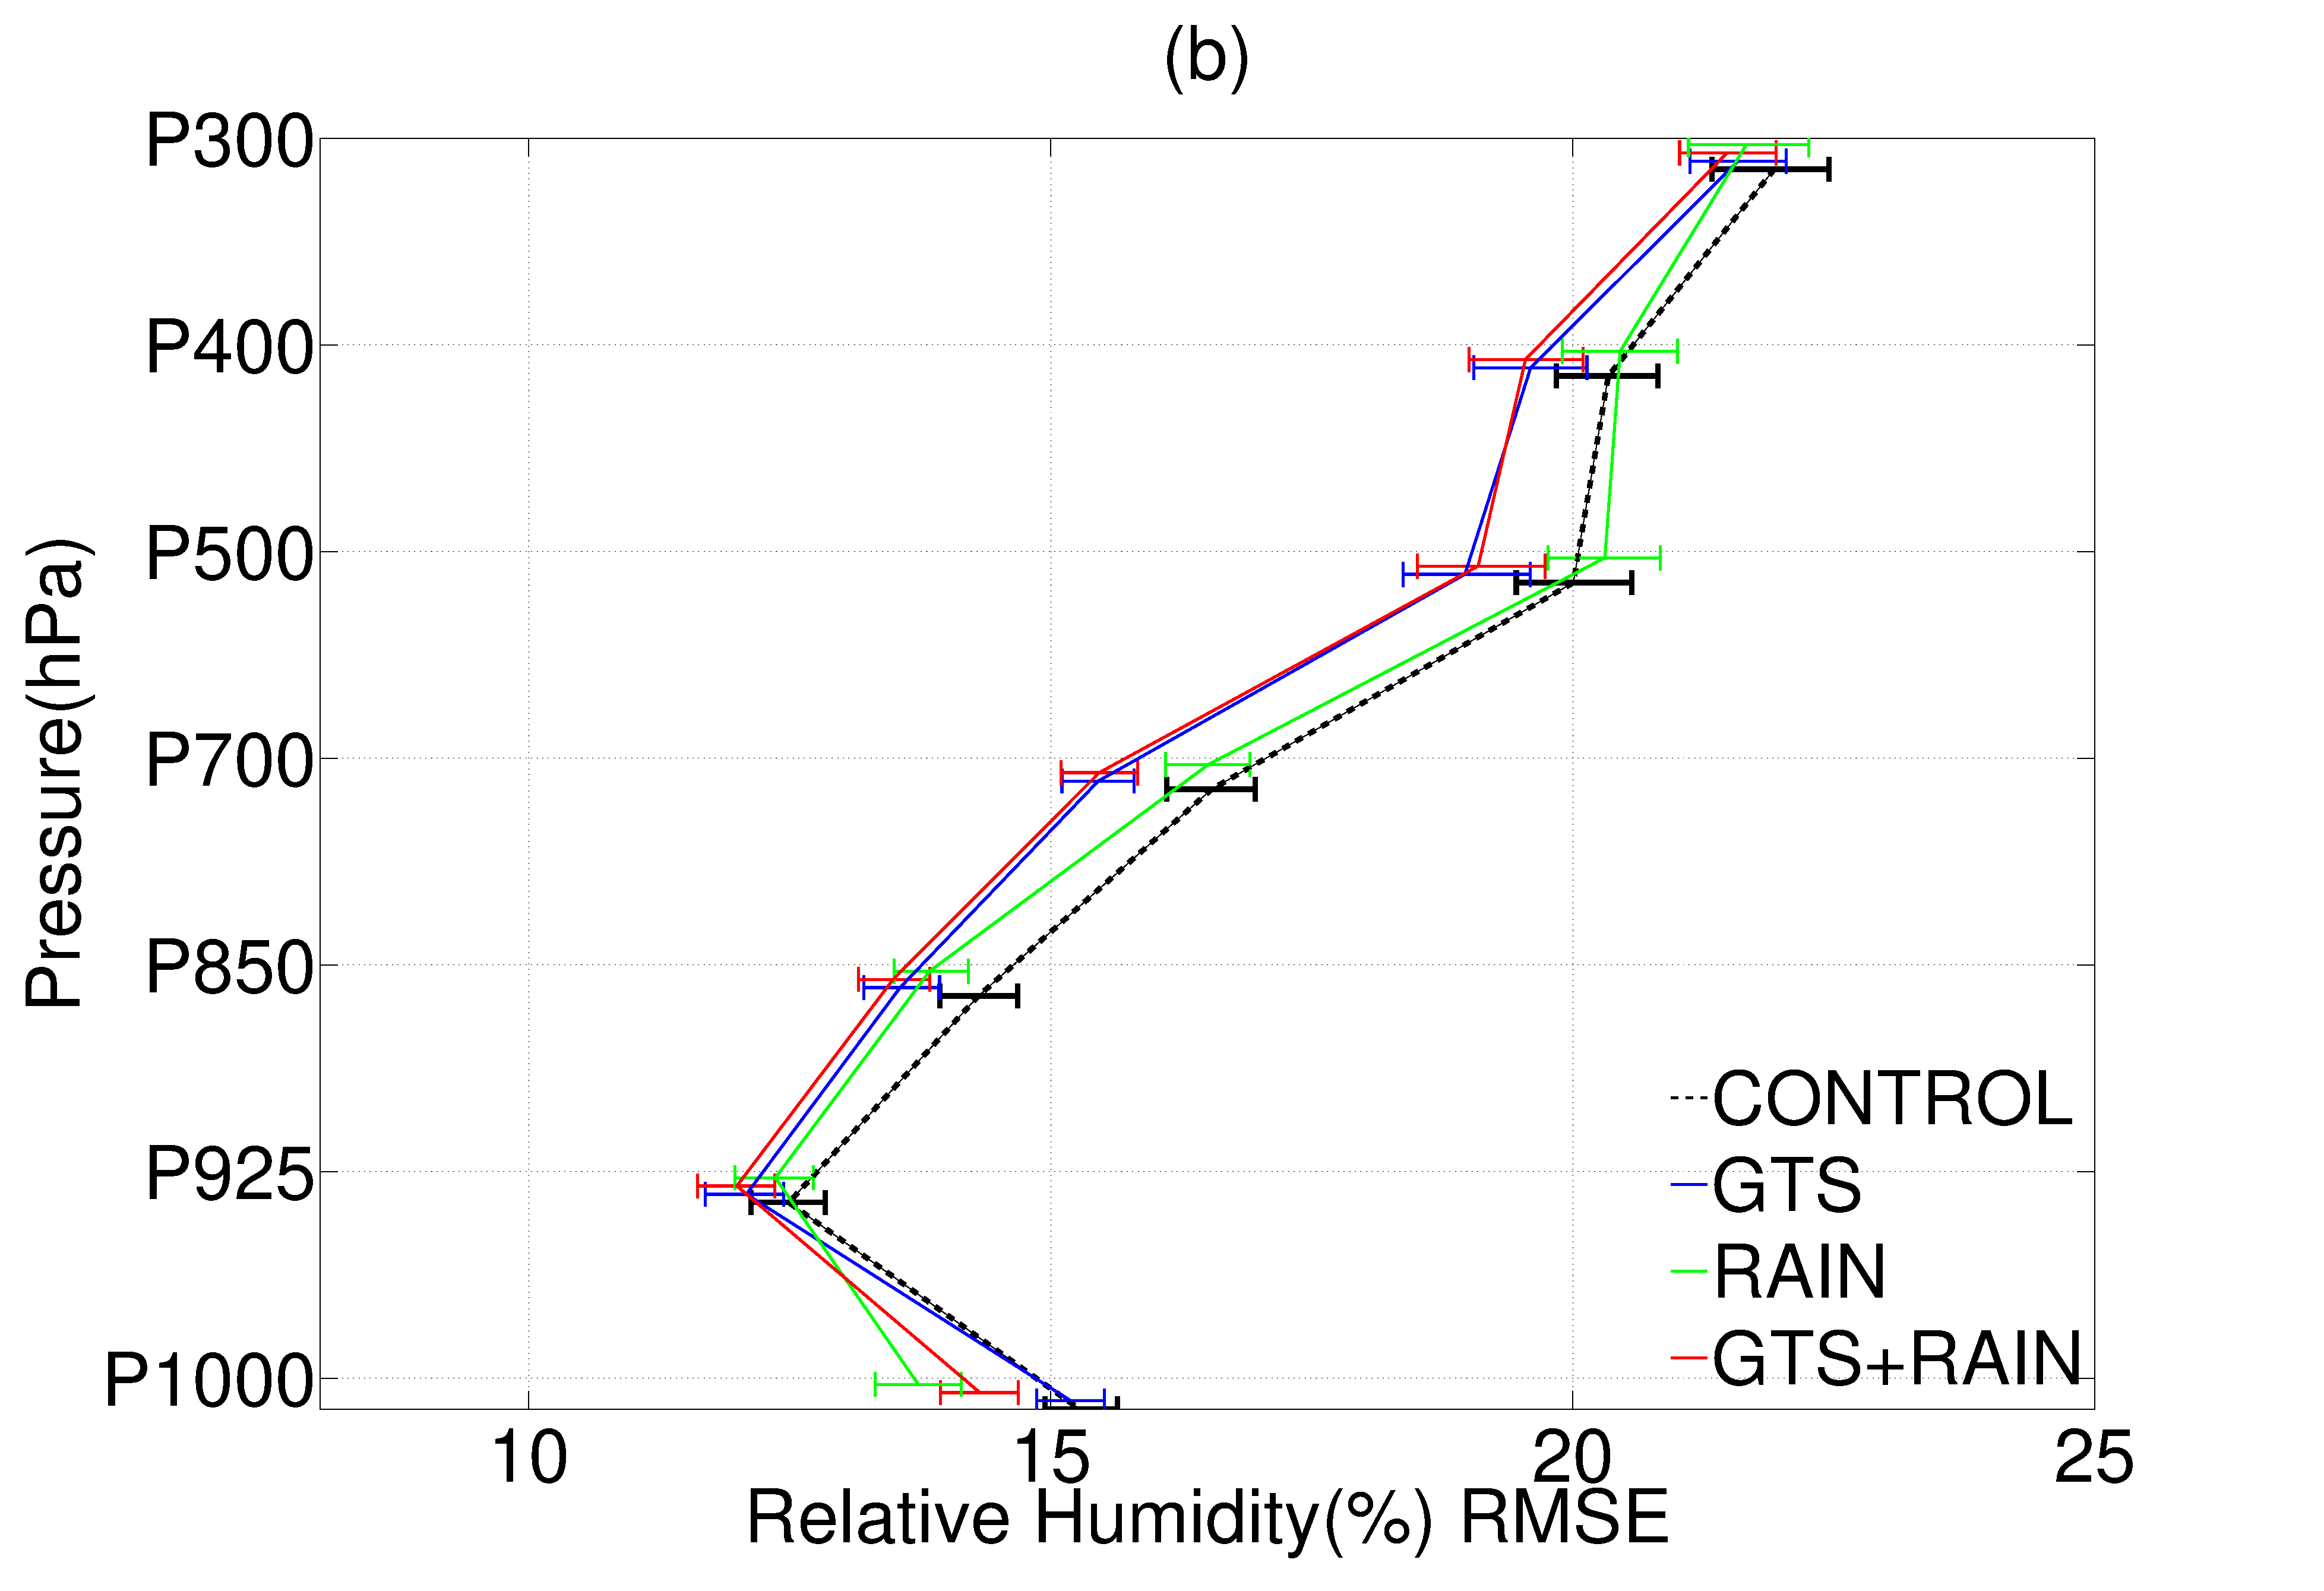
\includegraphics[width=19pc,angle=0]{rh_12.eps}\\
  \noindent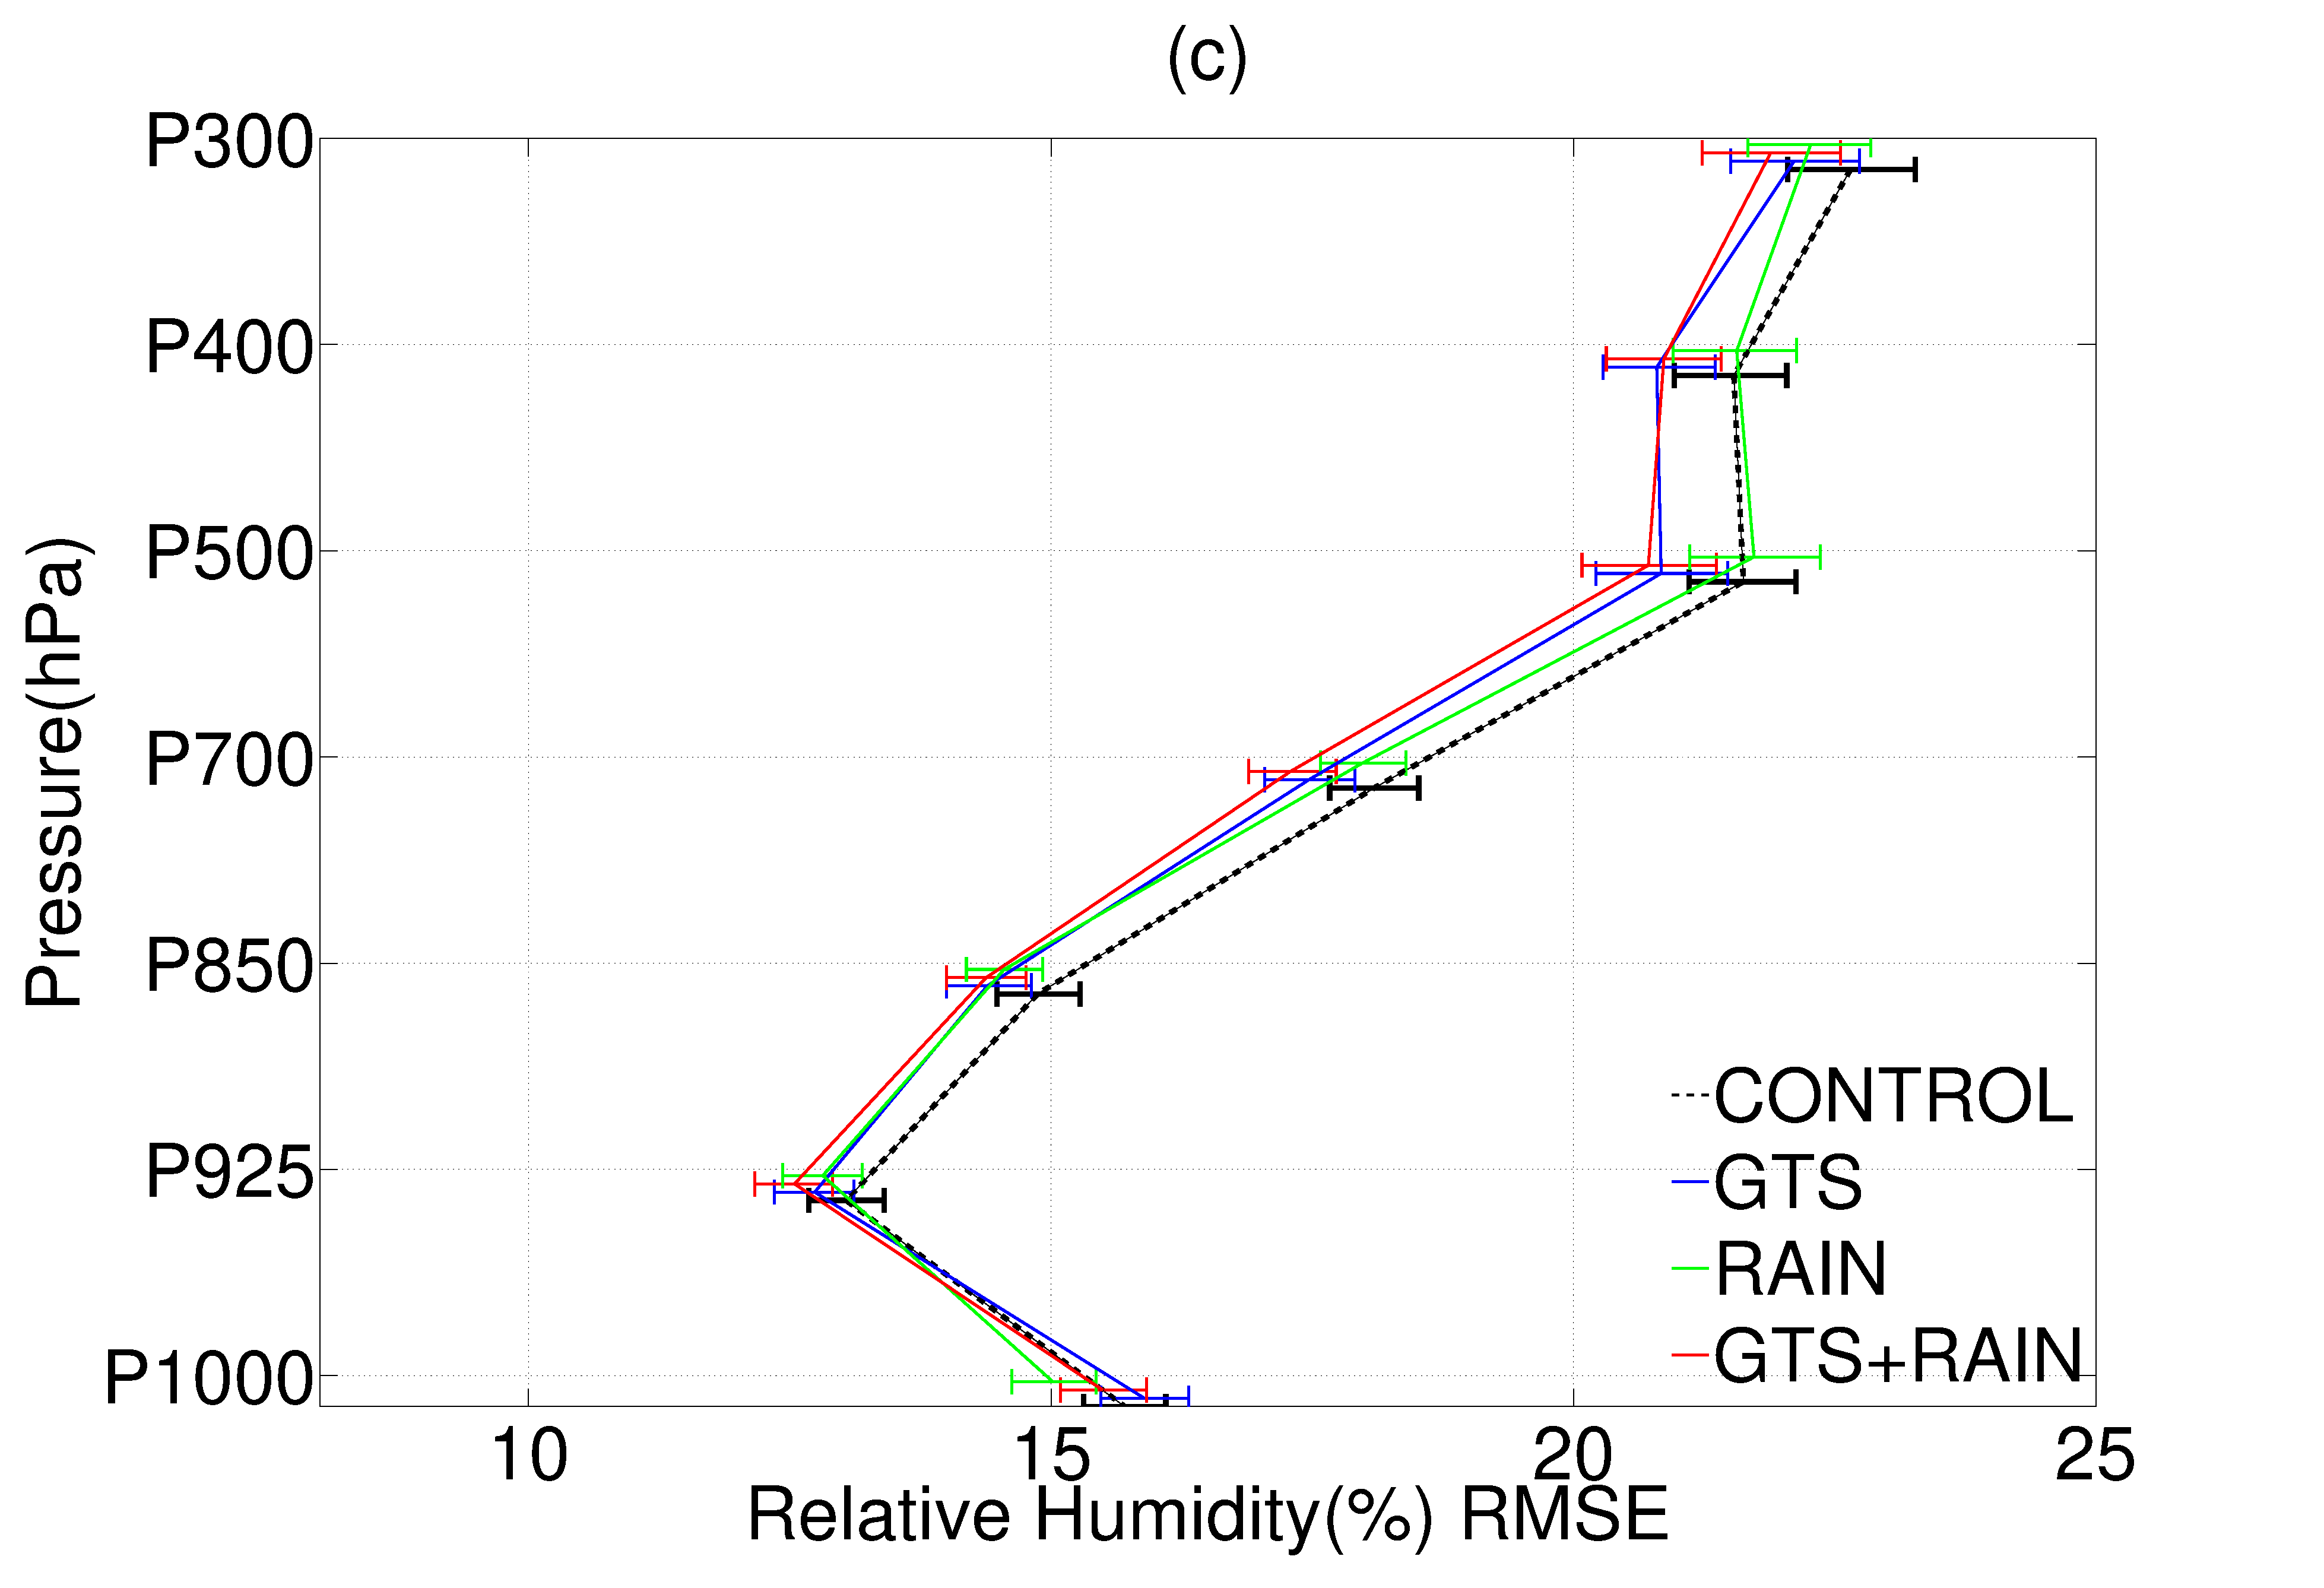
\includegraphics[width=19pc,angle=0]{rh_24.eps}\\  
   \caption{Same as Figure 1 but for relative humidity. }
 \label{f3}
\end{figure}

 \begin{figure}[!ht]\centering 
  \noindent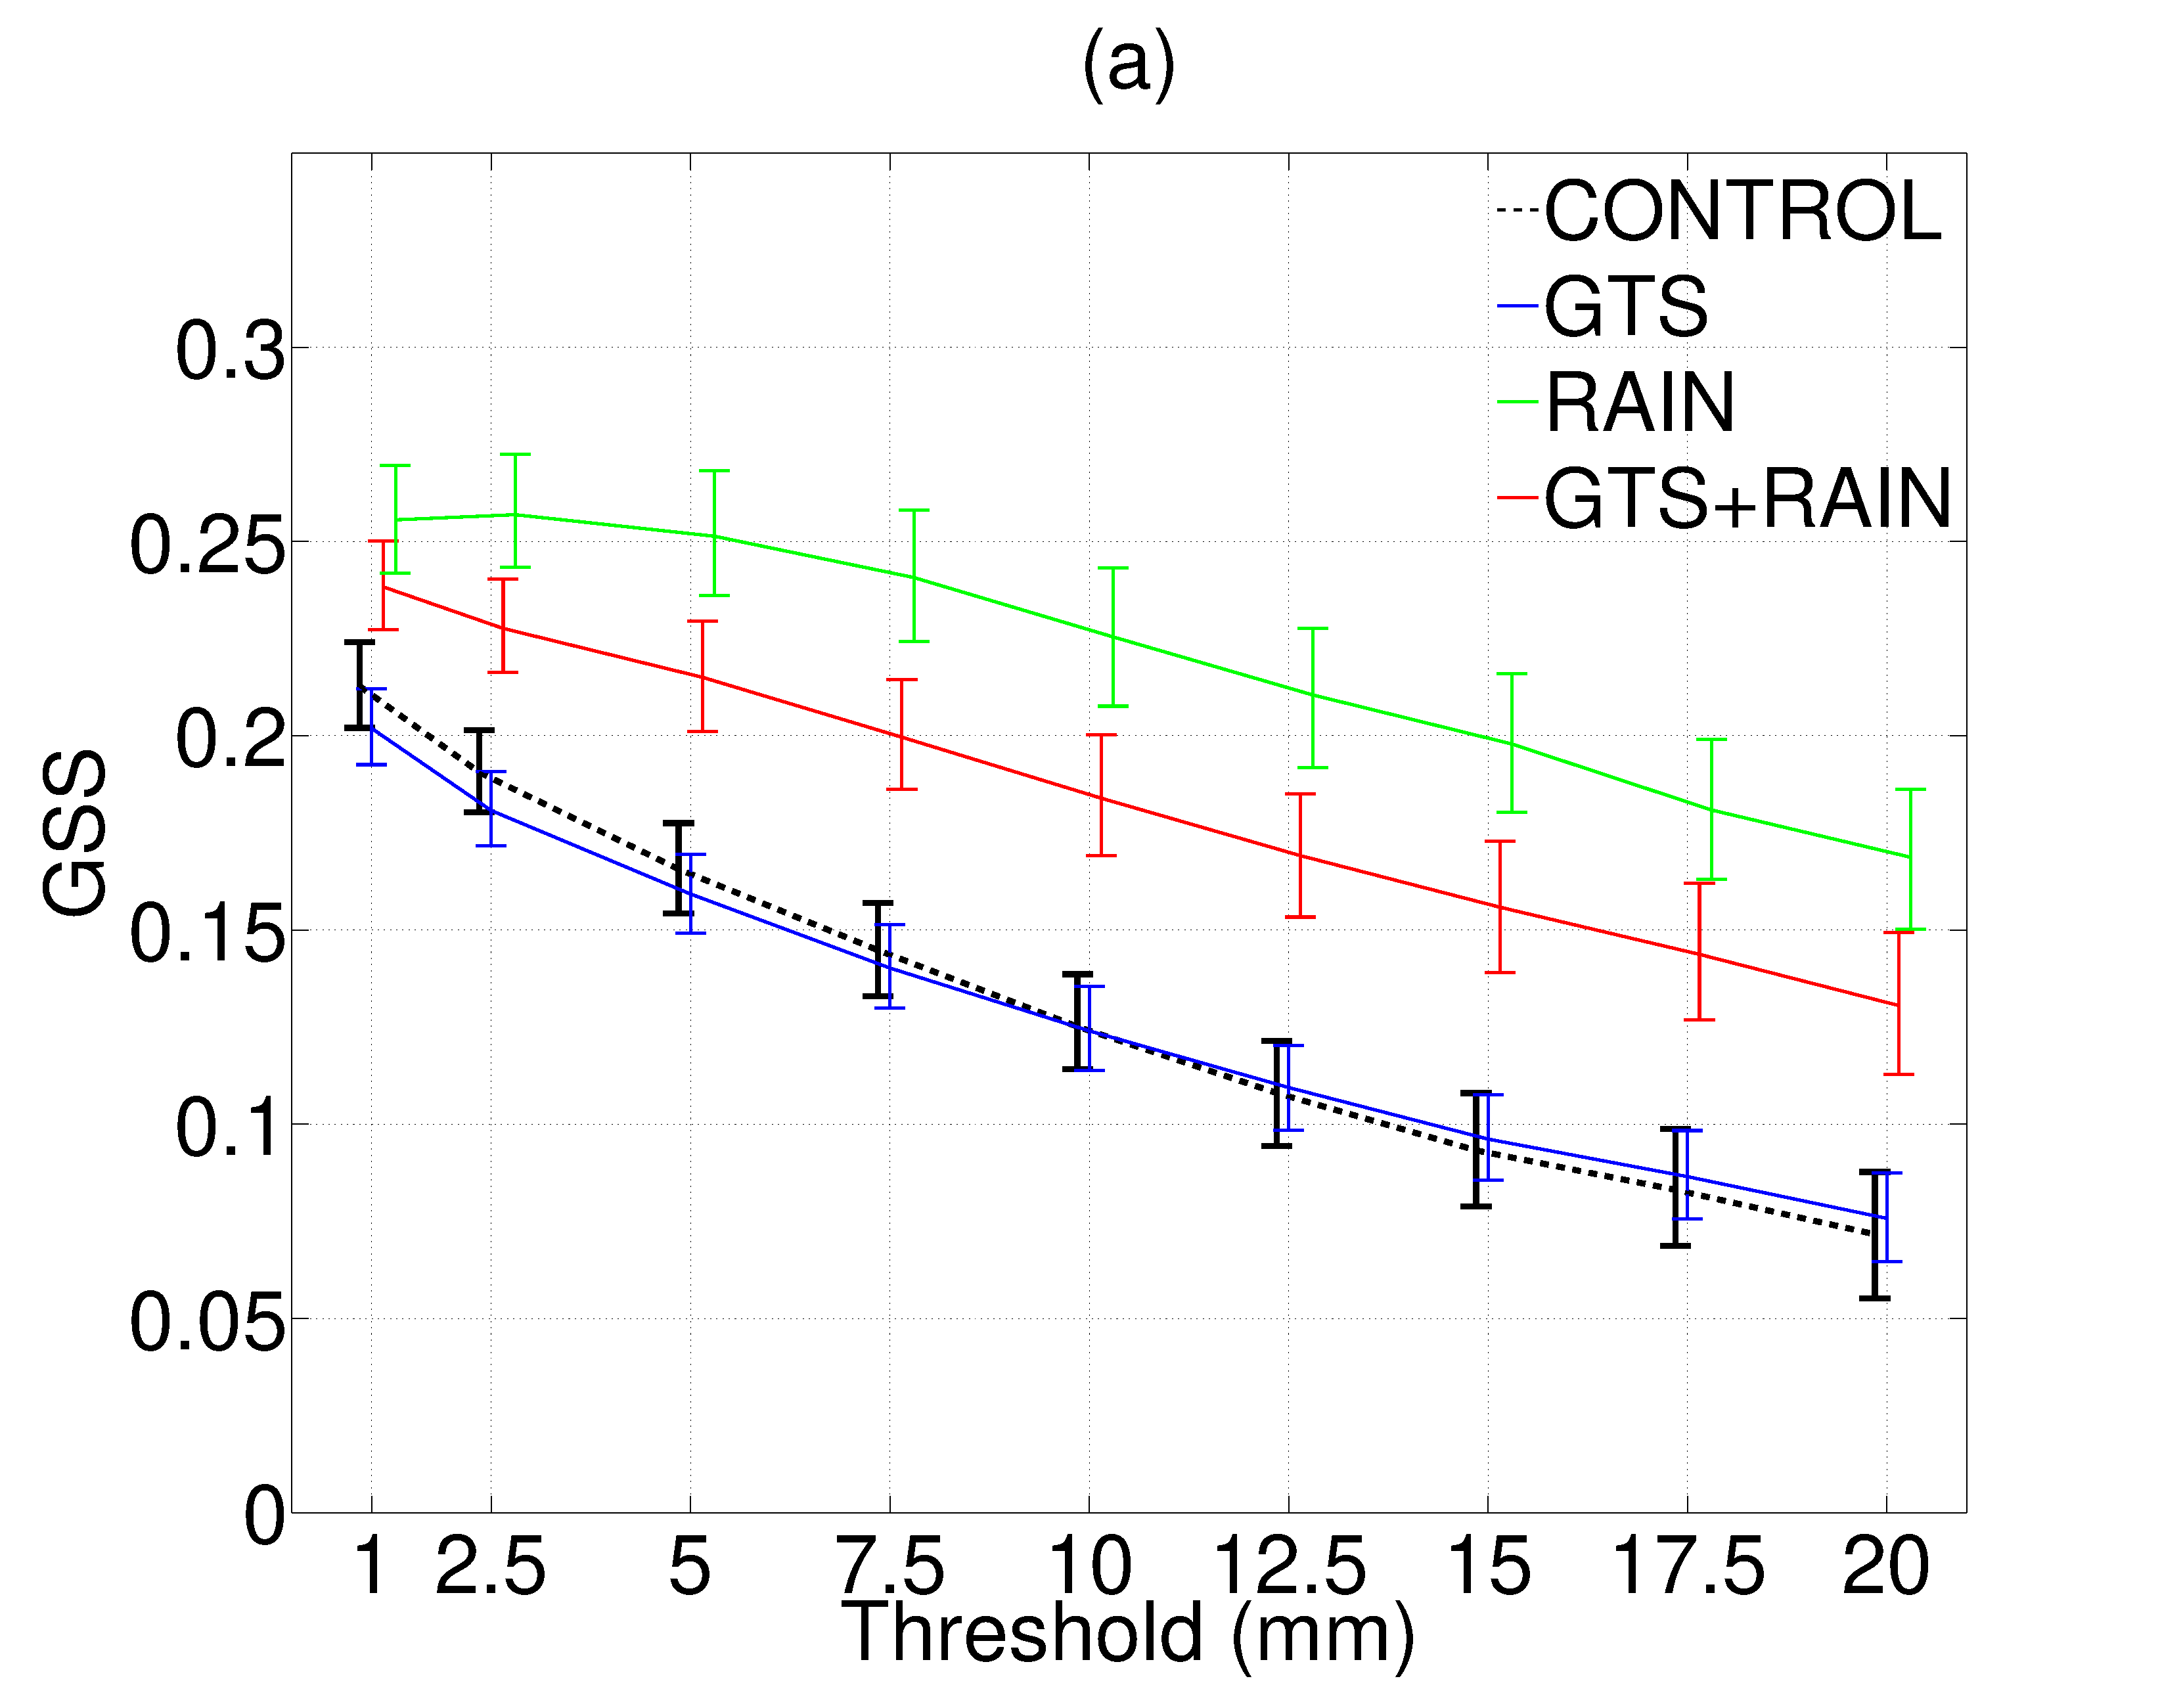
\includegraphics[width=27pc,angle=0]{GSS_06.eps}\\
  \noindent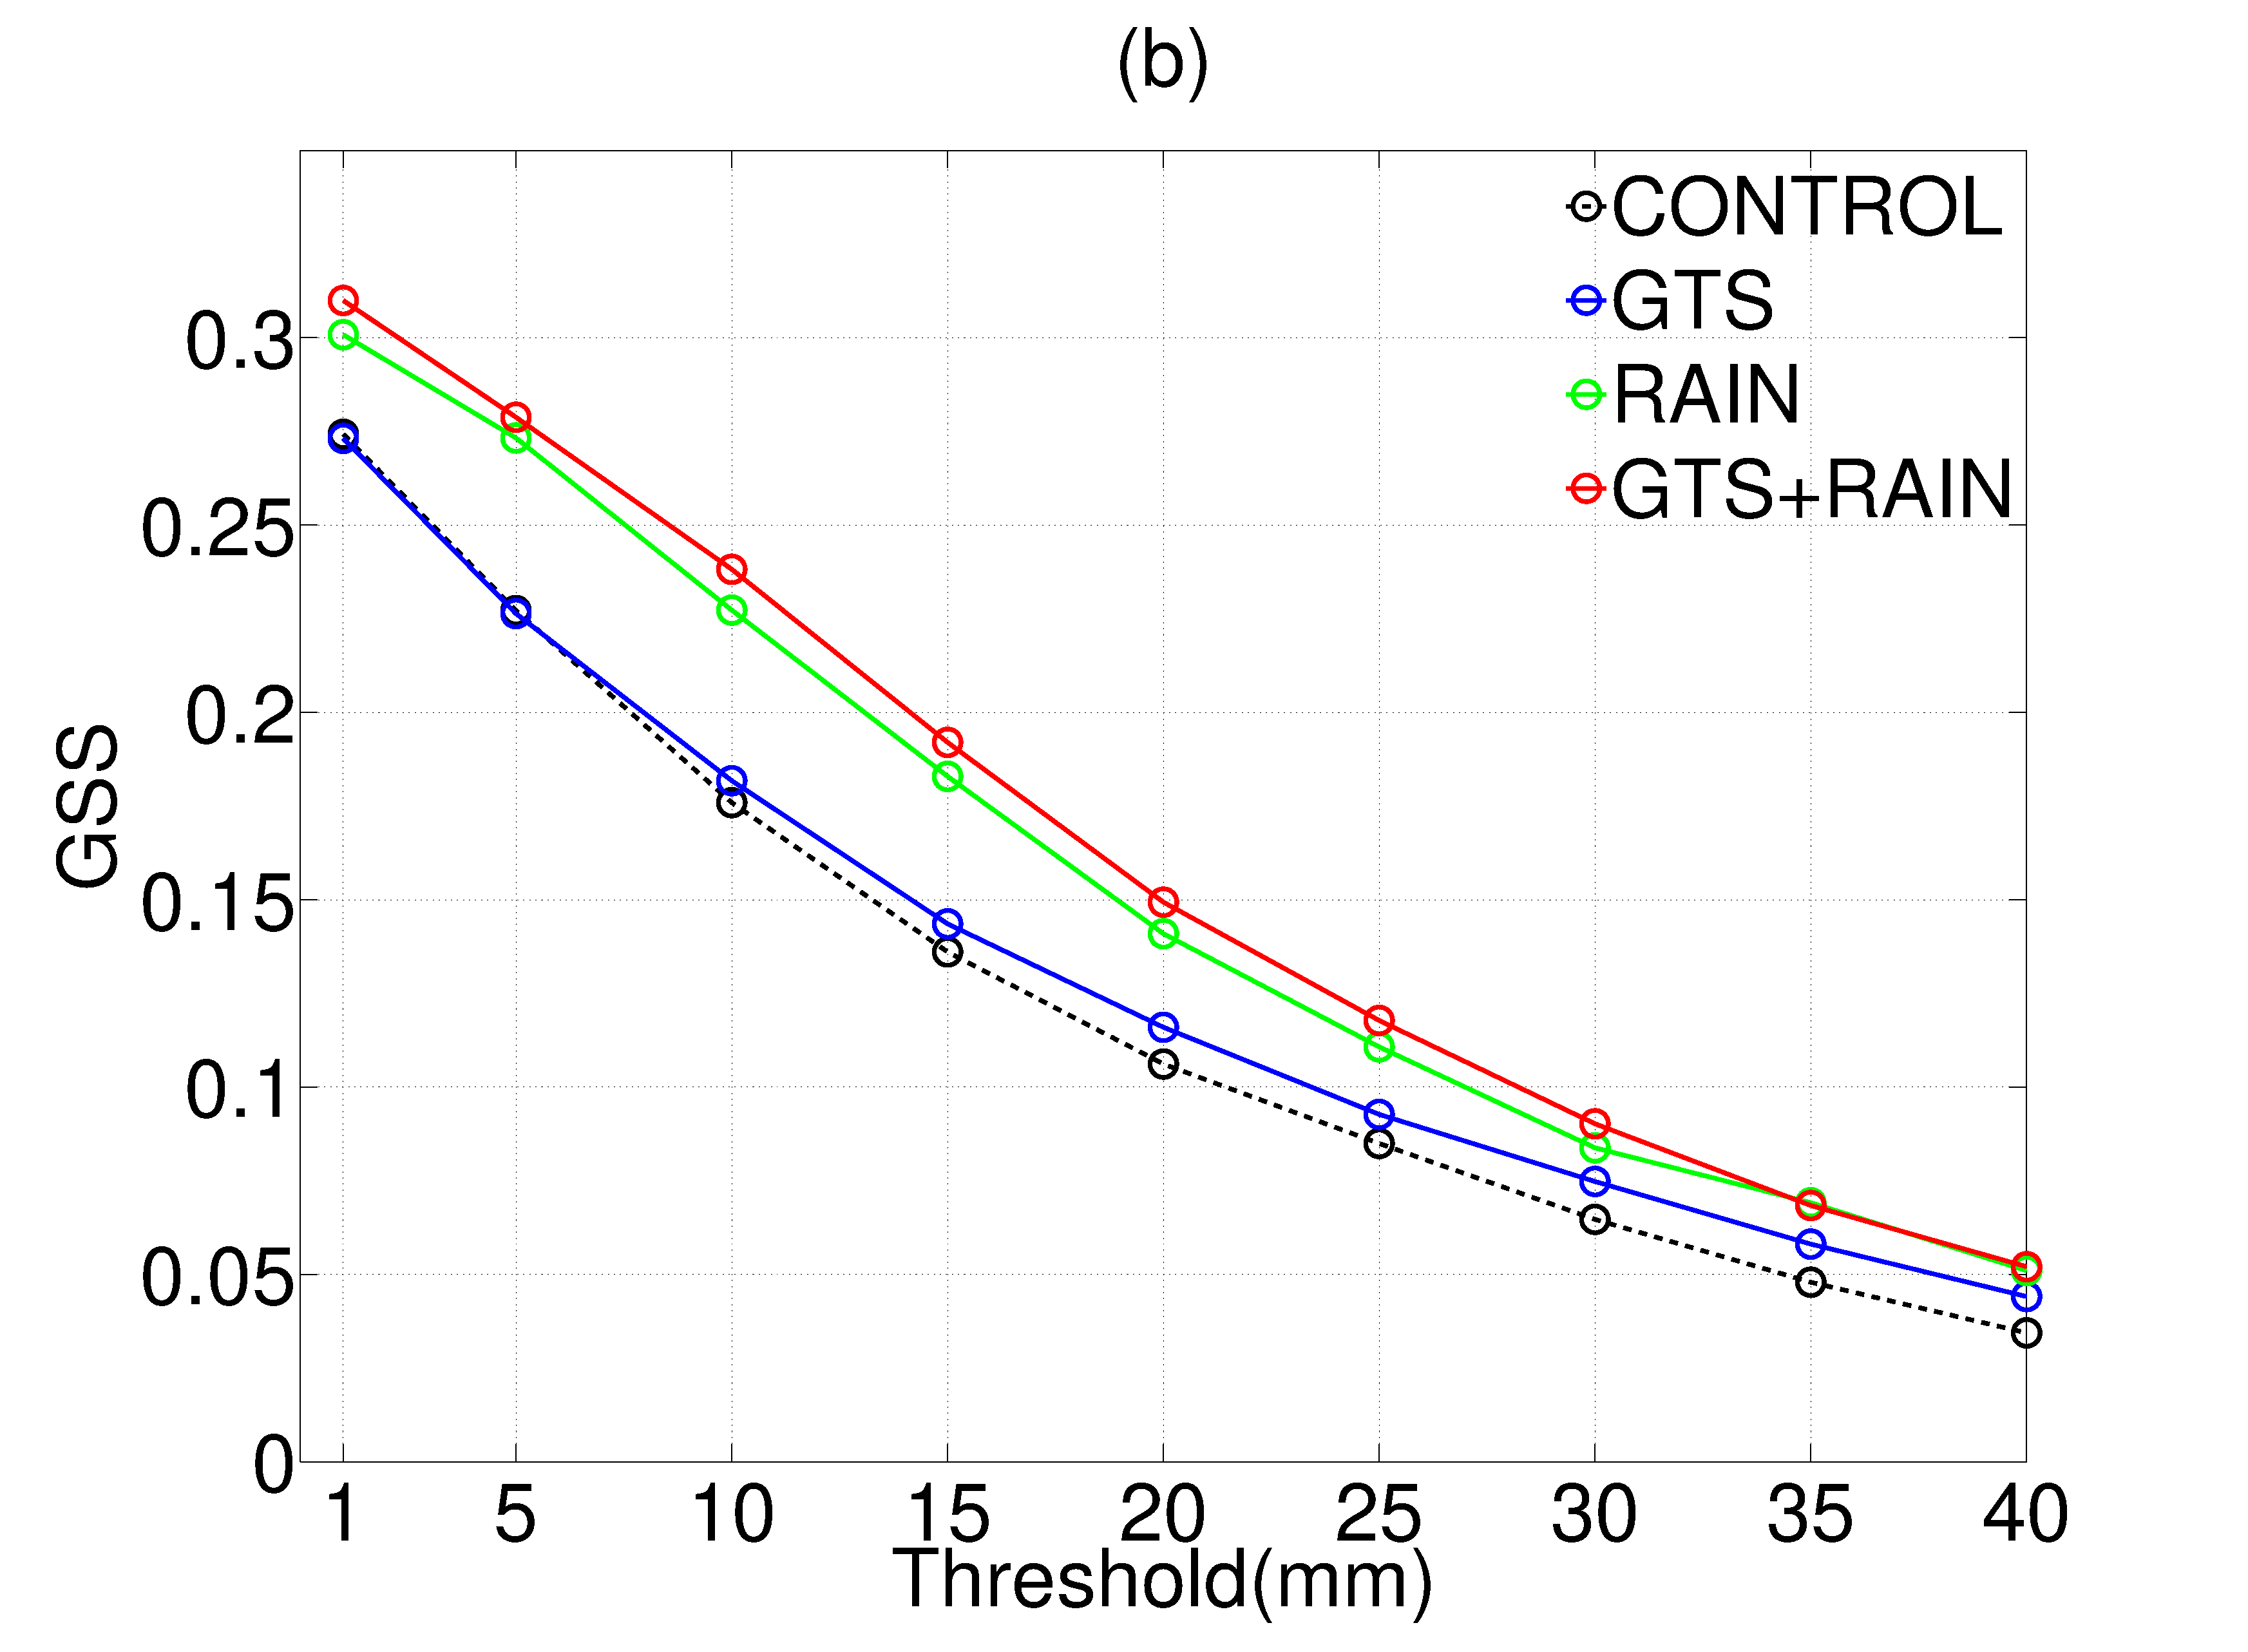
\includegraphics[width=27pc,angle=0]{GSS_12.eps}\\ 
  \caption{Threshold series of the GSS for 6-h (a), 12-h (b), 18-h (c), and 24-h (d) accumulated precipitation from the experiment CONTROL, GTS, RAIN, GTS+RAIN aggregated over 1-month period. The vertical bars represent the confidence intervals at the 95\% confidence level.}
   \label{f4}
\end{figure}
\begin{figure}[!ht]\centering
   \addtocounter{figure}{-1}   
  \noindent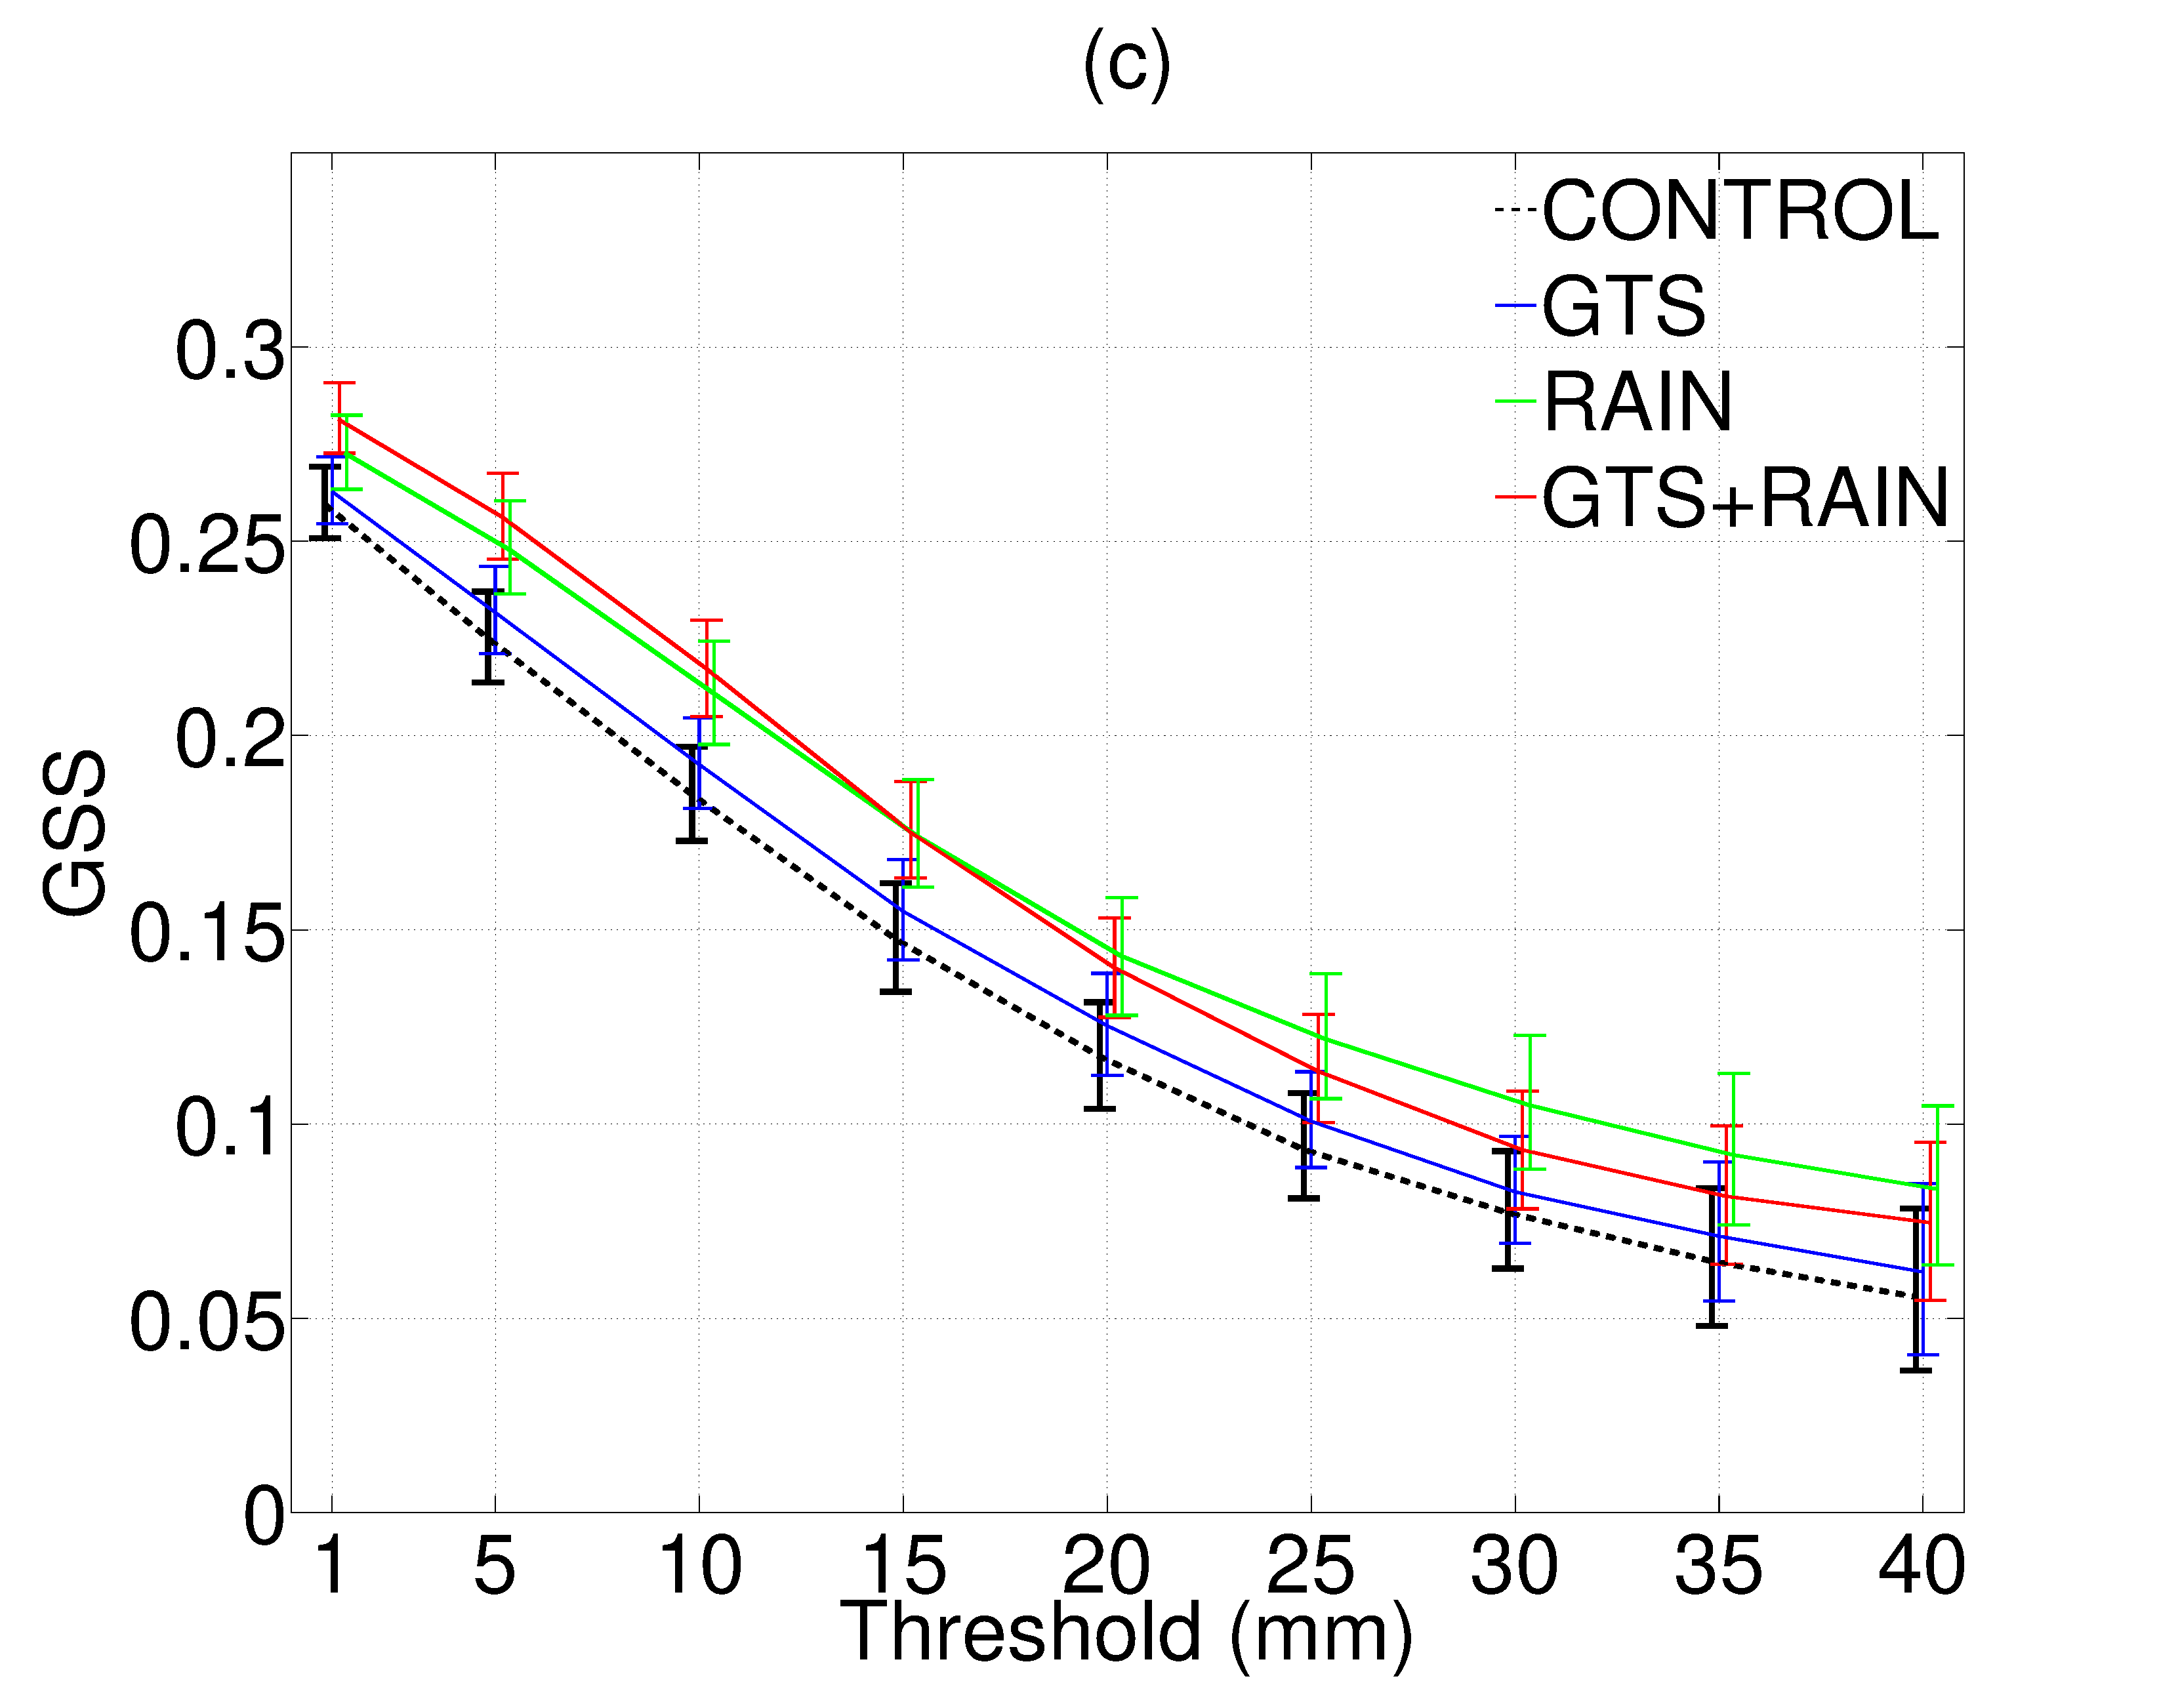
\includegraphics[width=27pc,angle=0]{GSS_18.eps}\\
  \noindent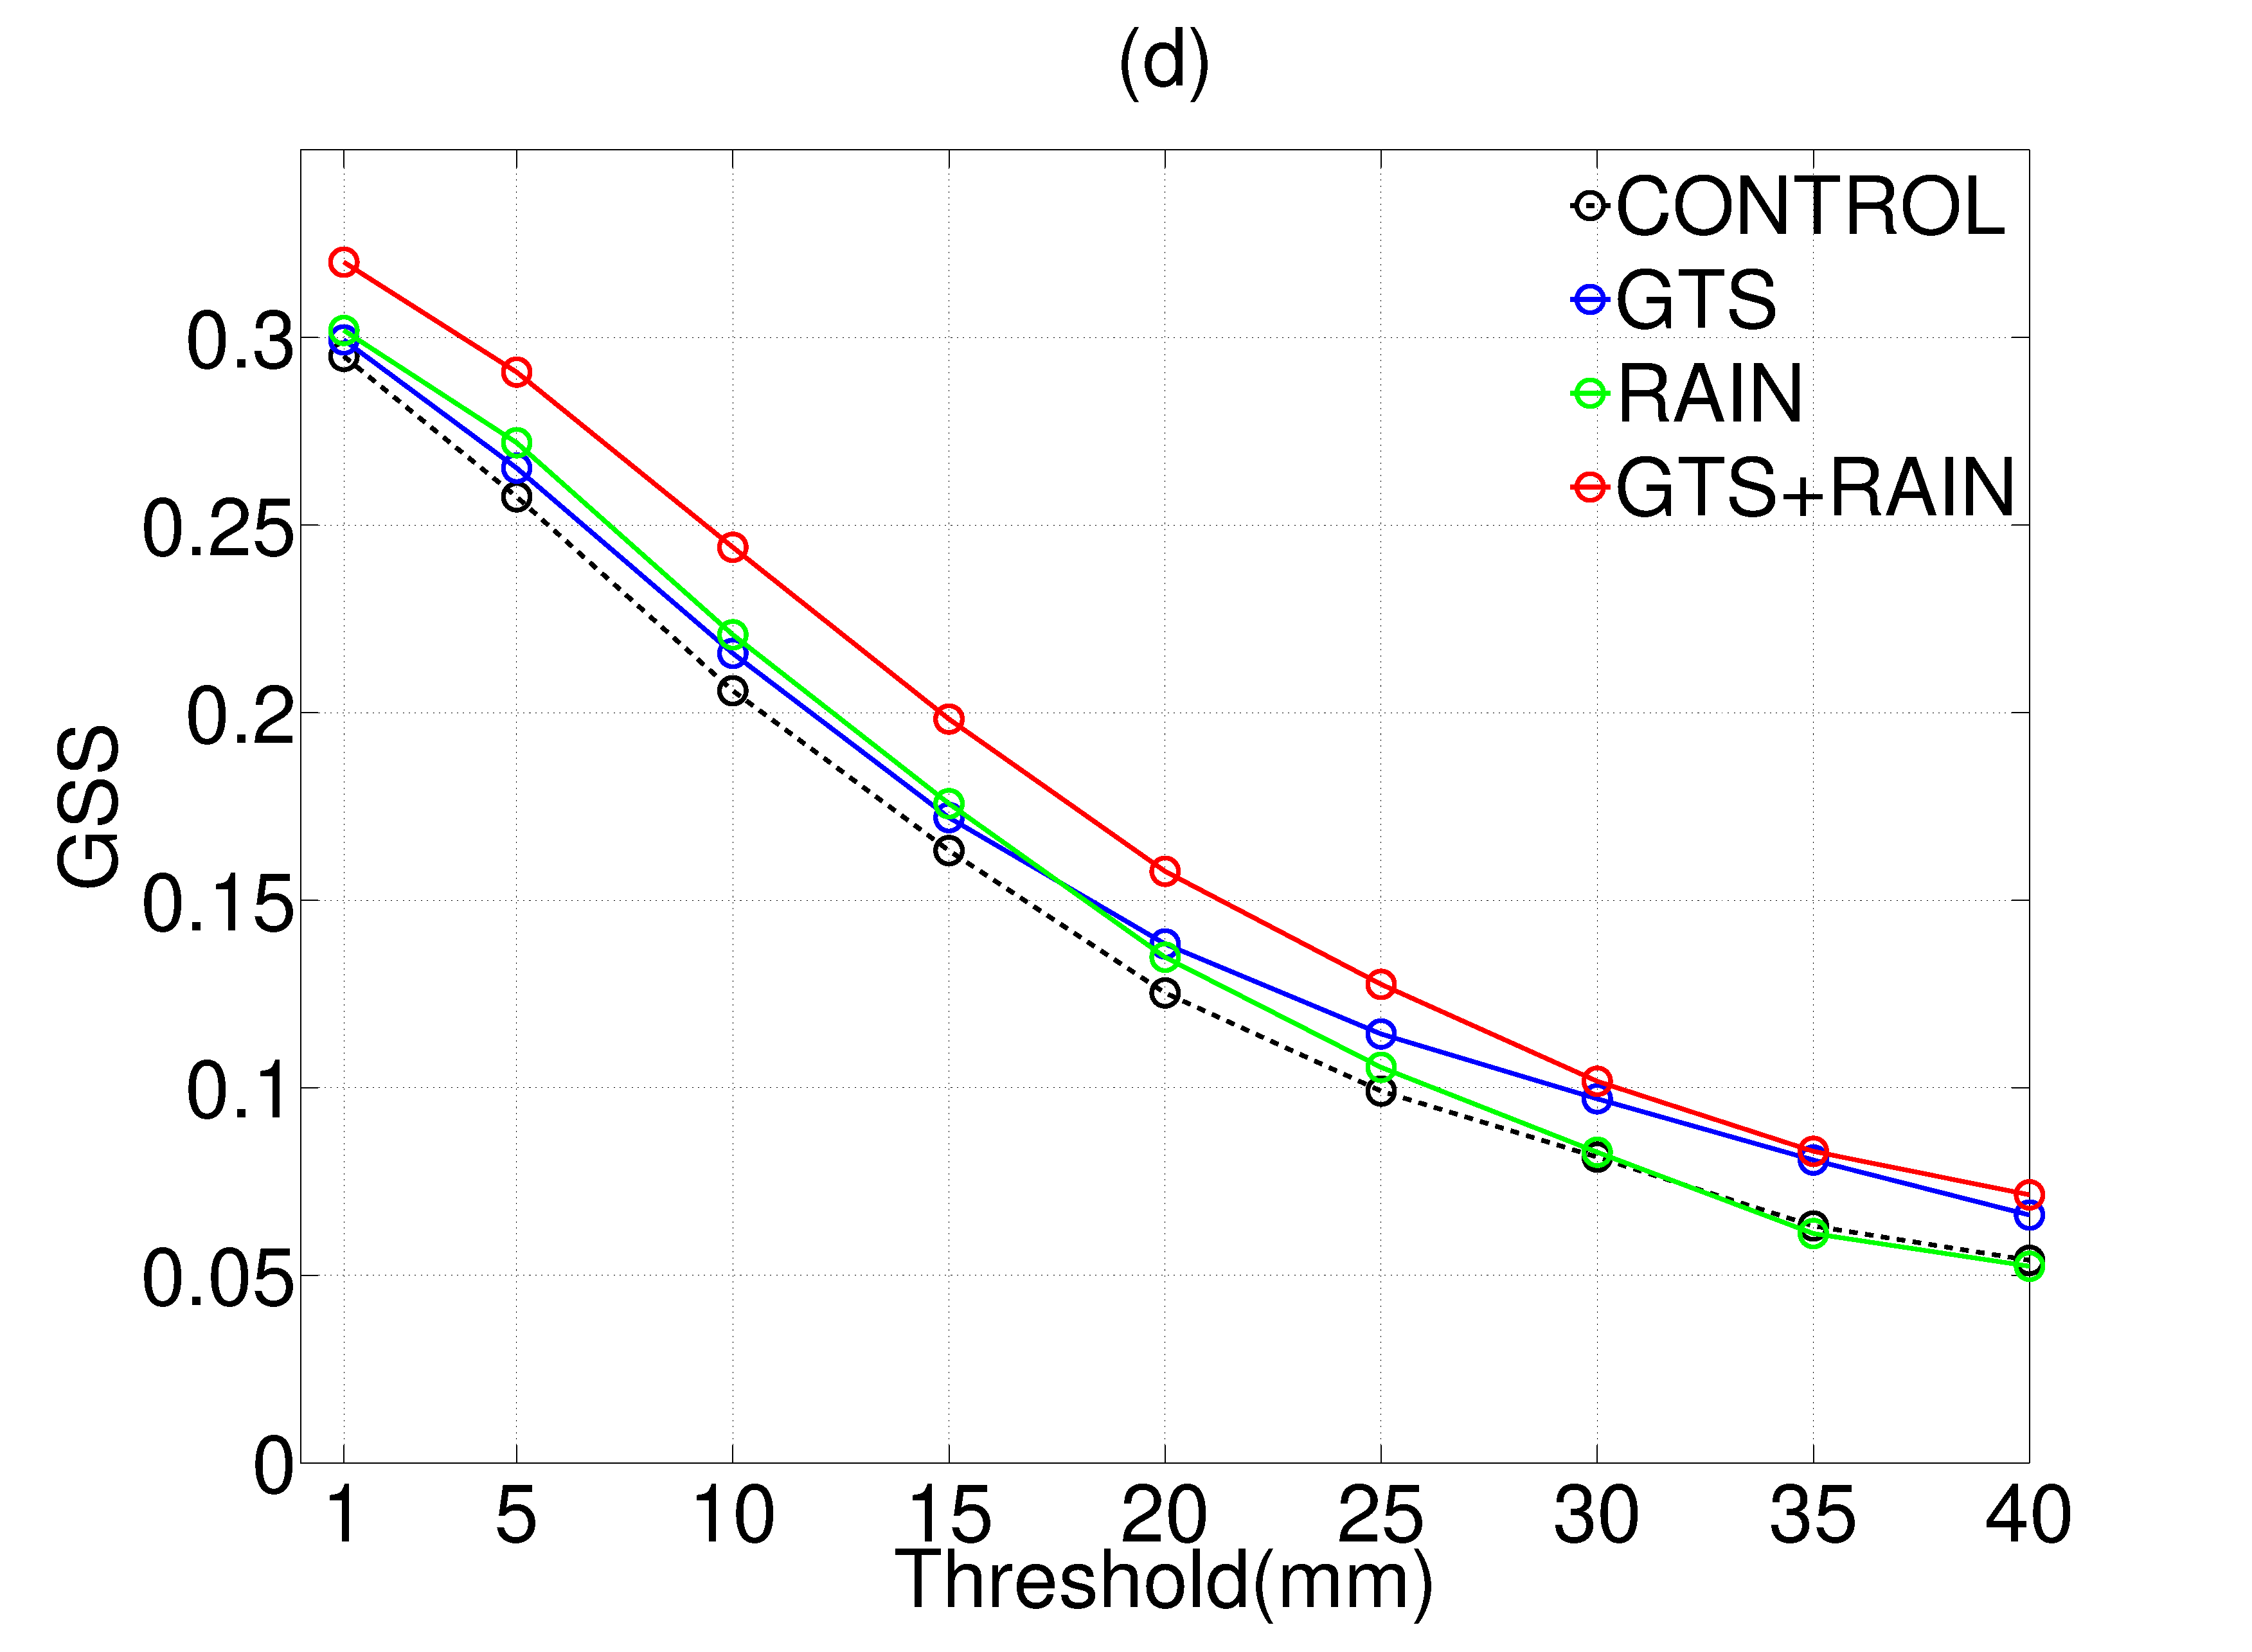
\includegraphics[width=27pc,angle=0]{GSS_24.eps}\\   
   \caption{continued}
   \label{f4}
\end{figure}

\begin{figure}
  \noindent\includegraphics[width=27pc,angle=0]{500hpa_850hpa.eps}\\
   \caption{500hpa (right) and 850hpa (left) geopotential height (blue solid line), temperature (red dashed line) and wind (in knots) at 0000UTC 9 June 2010. }
   \label{f5}
\end{figure}

\begin{figure}
  \noindent\includegraphics[width=27pc,angle=0]{obs.eps}\\
   \caption{NCEP Stage-IV 24-h accumulated precipitation (mm) valid at 0000 UTC 10 June 2010. The original precipitation accumulations are available on a 4-km resolution polar-stereographic grid. It has been regrided to 30 km lambert conformal grid. }
   \label{f6}
\end{figure}
 
 \begin{figure}[!ht]\centering 
   \noindent\includegraphics[width=27pc,angle=0]{diff_rh_1.eps}\\ 
  \caption{Analysis increment of relative humidity and analysis of geopotential height (blue solid line) and wind (in knots) by (a)GTS, (b)RAIN and (c)GTS+RAIN at 850 hPa at 0000 UTC 9 June.}
   \label{f7}
\end{figure}
\begin{figure}[!ht]\centering
   \addtocounter{figure}{-1}   
   \noindent \includegraphics[width=27pc,angle=0]{diff_rh_2.eps}\\  
   \caption{continued}
   \label{f7}
\end{figure}
 
  \begin{figure}
  \noindent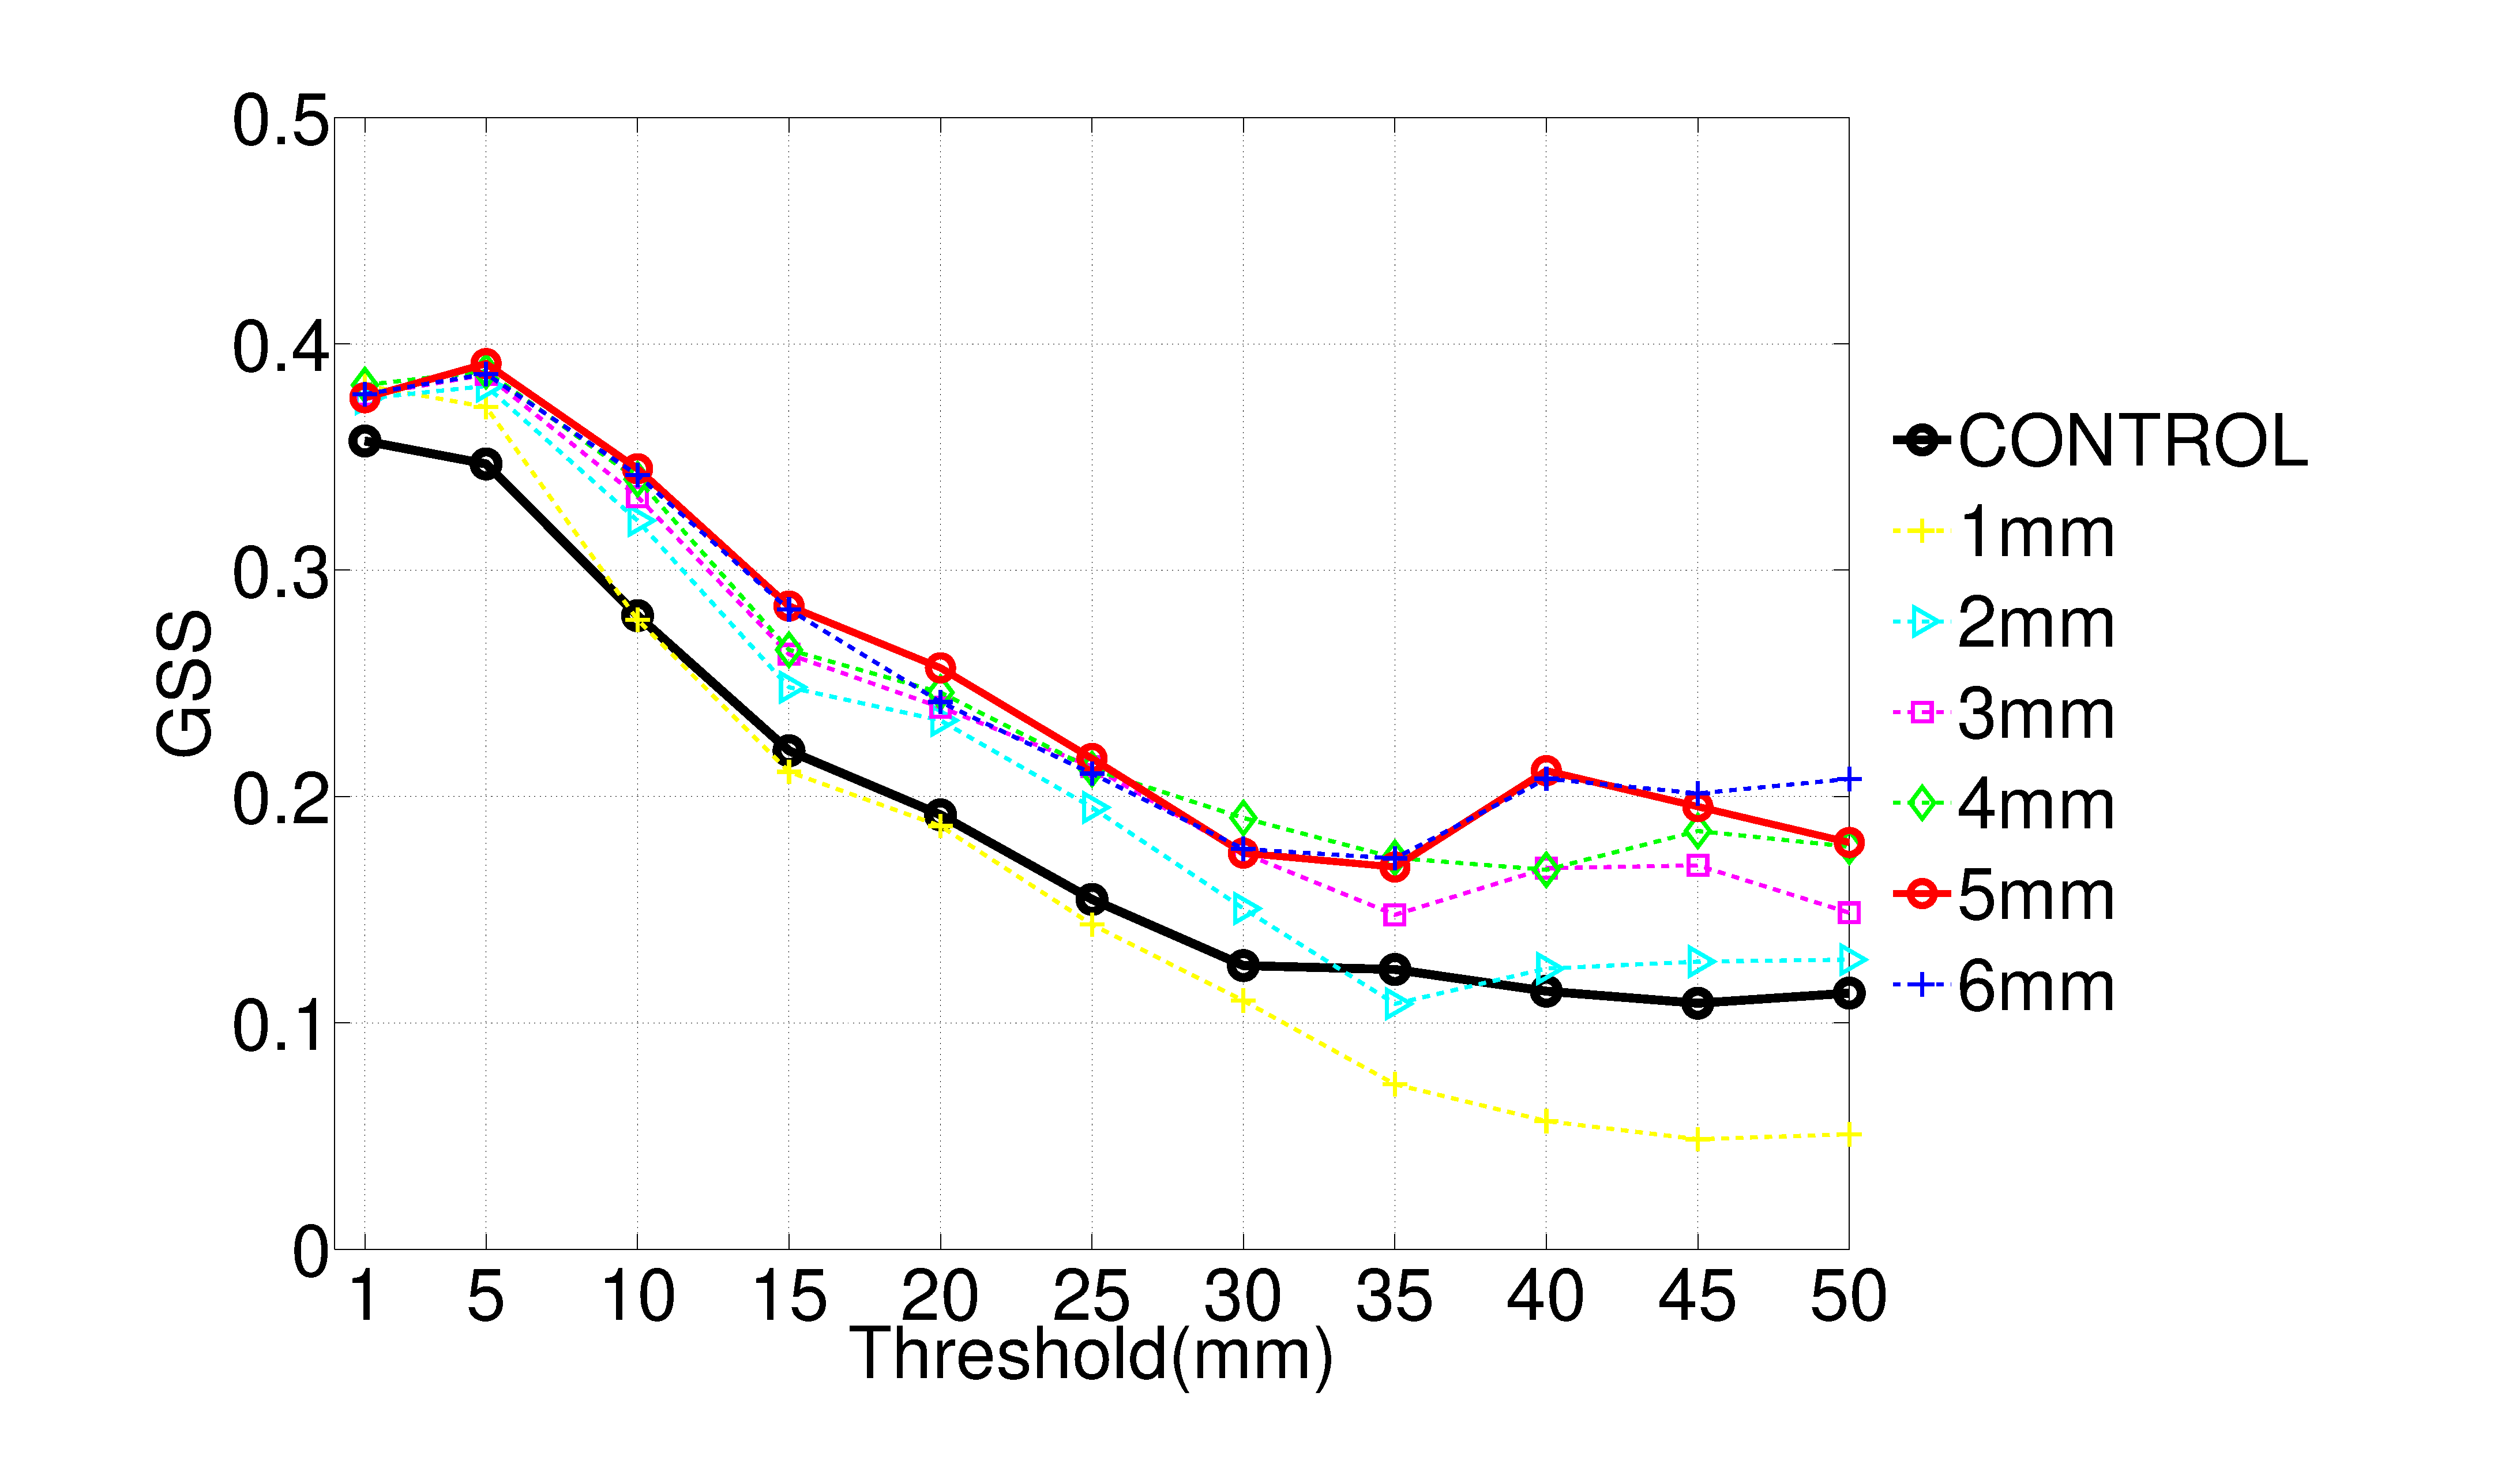
\includegraphics[width=33pc,angle=0]{GSS_24_sensitive_error.eps}\\
   \caption{Threshold series of the GSSs for 24-h accumulated precipitation using 1mm-6mm observation error and CONTROL valid at 0000 UTC 10 June 2010.}
   \label{f8}
\end{figure}
 
   \begin{figure}
  \noindent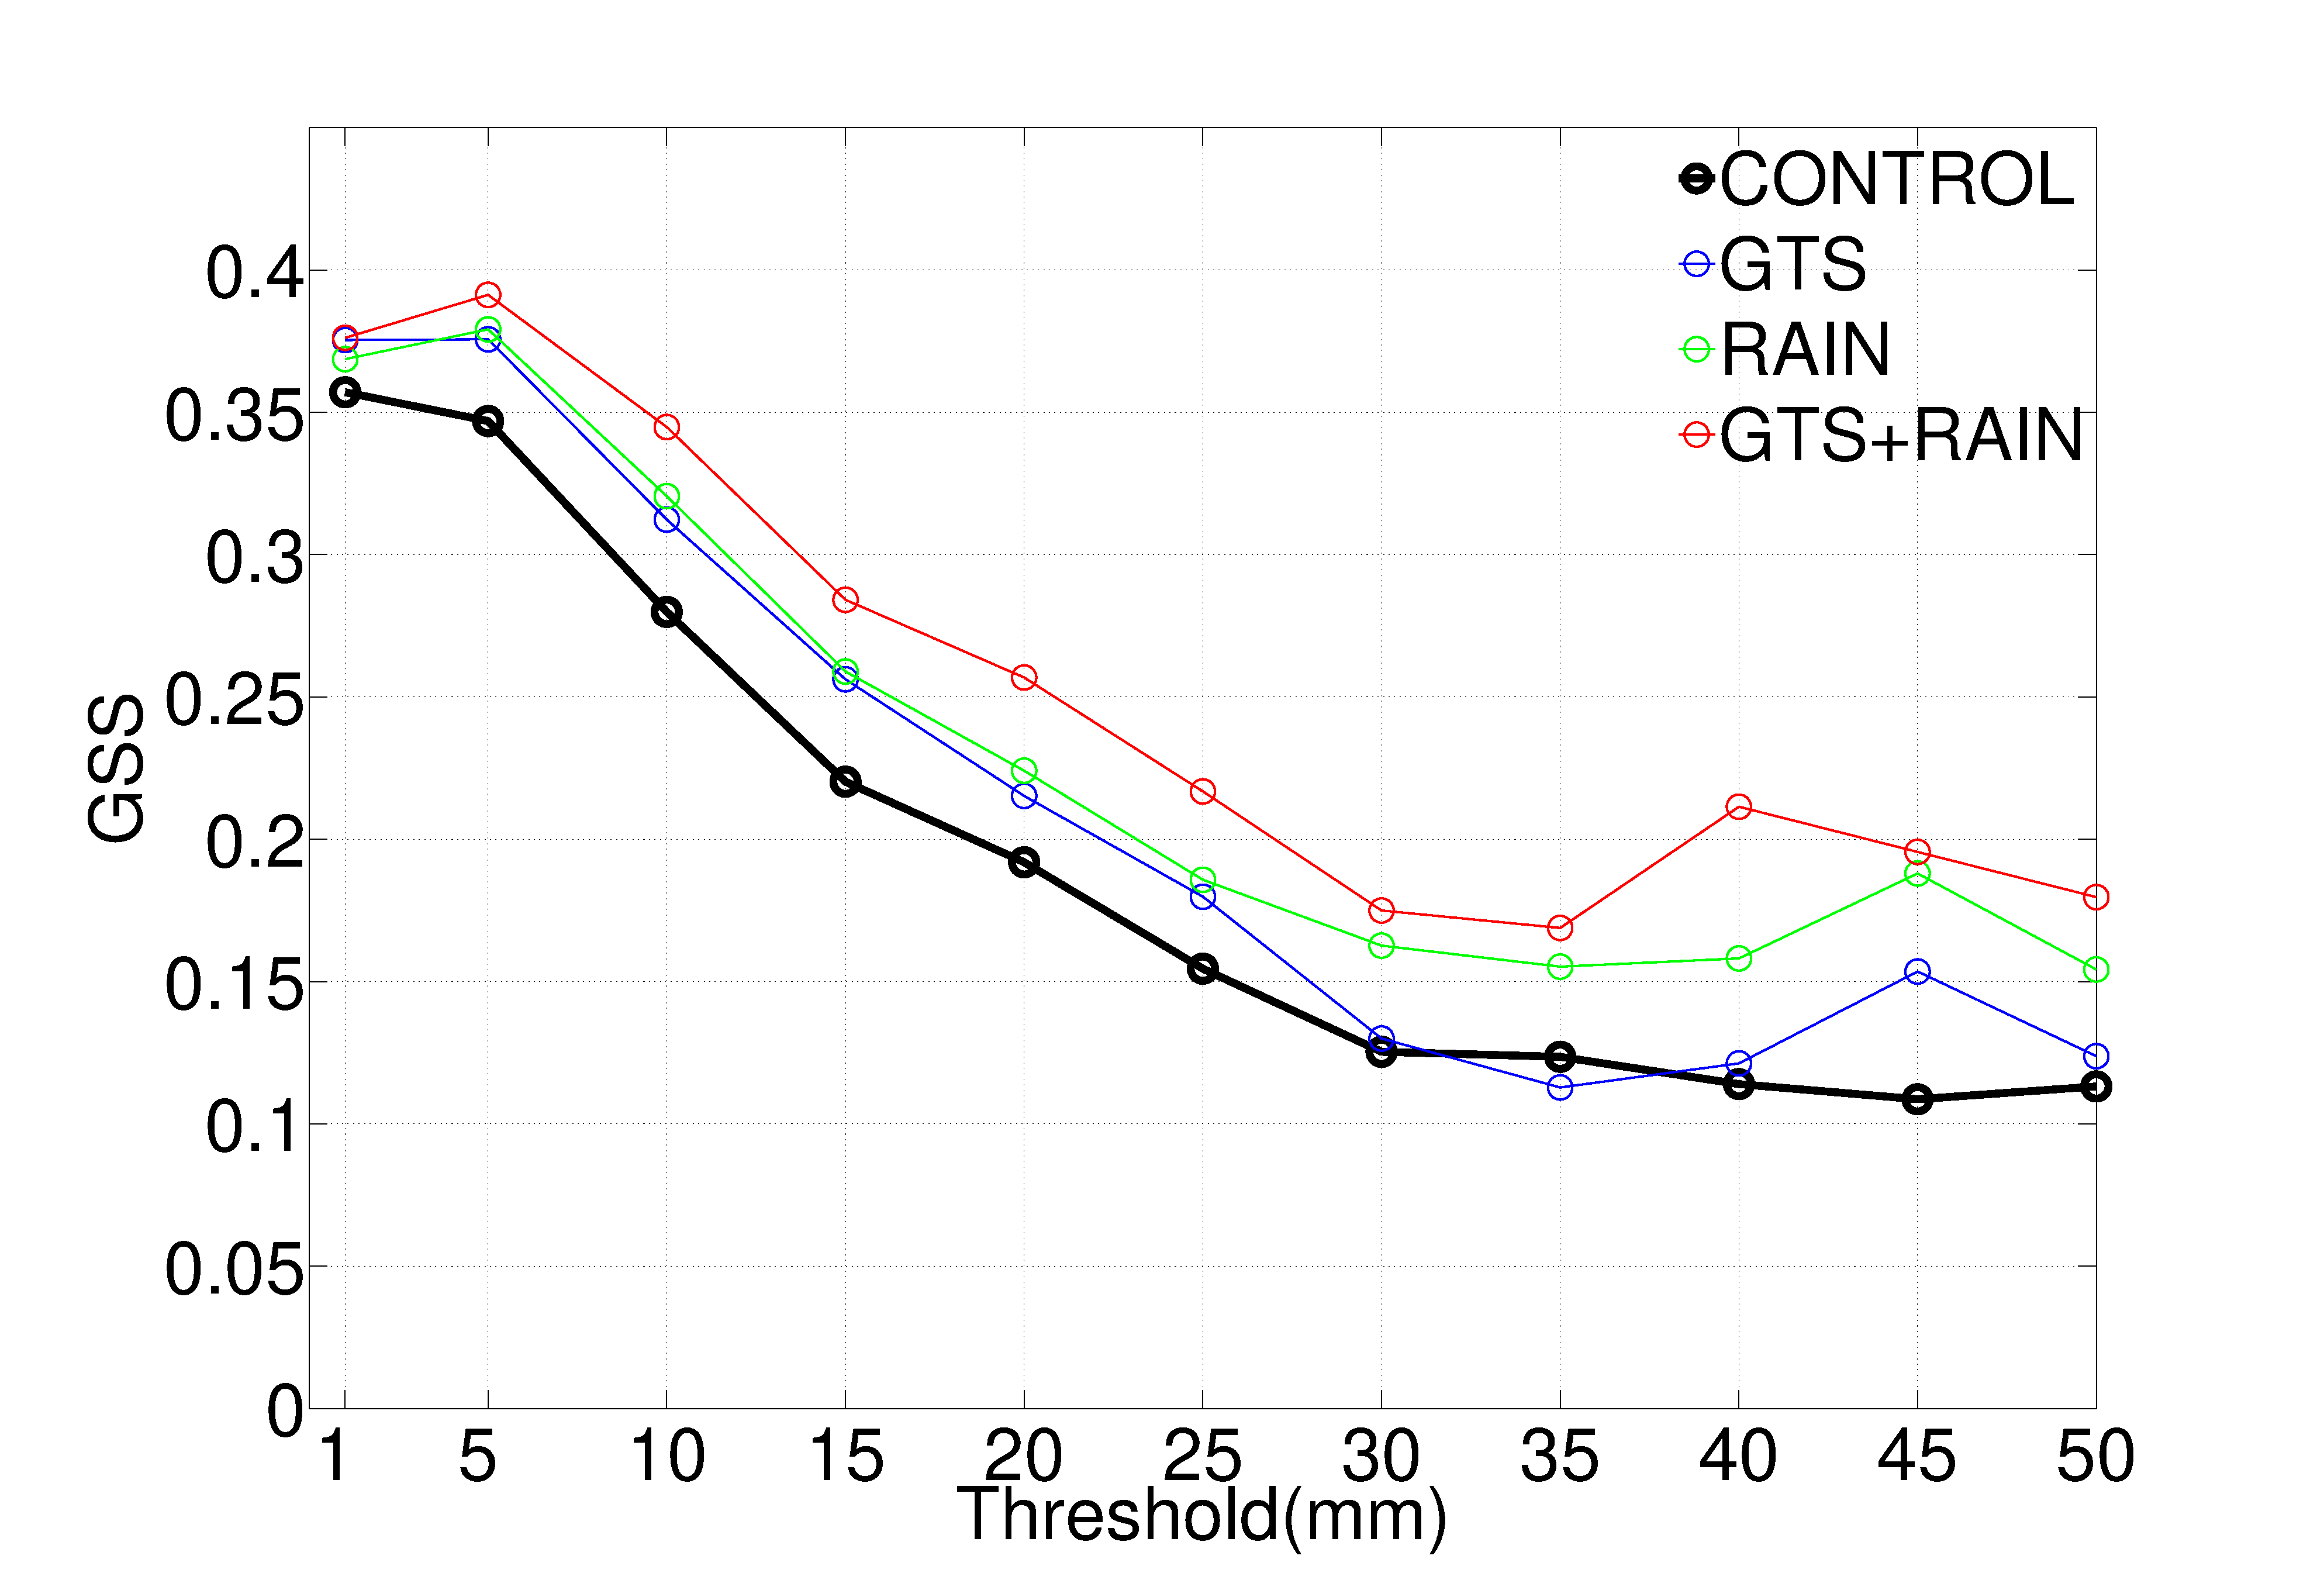
\includegraphics[width=29pc,angle=0]{gss_singlecase.eps}\\
   \caption{Threshold series of the GSS for 24-h accumulated precipitation from the experiment CONTROL, GTS, RAIN, GTS+RAIN valid at 0000 UTC 10 June 2010. }
   \label{f9}
\end{figure}
 
  \begin{figure}[!ht]\centering 
   \noindent\includegraphics[width=27pc,angle=0]{control_1.eps}\\ 
   \noindent\includegraphics[width=27pc,angle=0]{gts_1.eps}\\    
  \caption{24-h accumulated precipitation (mm) valid at 0000 UTC 10 June 2010. (a) CONTROL (b) GTS (c) RAIN (d) GTS+RAIN.}
   \label{f10}
\end{figure}
\begin{figure}[!ht]\centering
   \addtocounter{figure}{-1}   
   \noindent \includegraphics[width=27pc,angle=0]{rain_1.eps}\\  
   \noindent \includegraphics[width=27pc,angle=0]{gts_rain_1.eps}\\     
   \caption{continued}
   \label{f10}
\end{figure}
 
%and caption is shown above. Standard figure sizes are 19 (one column), 27, 33, and 39 (two columns) picas

%%%%%%%%%%%%%%%%%%%%%%%%%%%%%%%%%%%%%%%%%%%%%%%%%%%%%%%%%%%%%%%%%%%%%
% ACKNOWLEDGMENTS
%%%%%%%%%%%%%%%%%%%%%%%%%%%%%%%%%%%%%%%%%%%%%%%%%%%%%%%%%%%%%%%%%%%%%
\begin{acknowledgment}
The National Center for Atmospheric Research is sponsored by the National Science Foundation. This work is supported by the Air Force Weather Agency.
The authors thank John Halley Gotway and Tatiana Burek from the Developmental Testbed Center for their help with METViewer.
We also thank Michael Kavulich (NCAR) for improving the English in the manuscript.
\end{acknowledgment}


%%%%%%%%%%%%%%%%%%%%%%%%%%%%%%%%%%%%%%%%%%%%%%%%%%%%%%%%%%%%%%%%%%%%%
% REFERENCES
%%%%%%%%%%%%%%%%%%%%%%%%%%%%%%%%%%%%%%%%%%%%%%%%%%%%%%%%%%%%%%%%%%%%%
% Create a bibliography directory and place your .bib file there.
\ifthenelse{\boolean{dc}}
{}
{\clearpage}
\bibliographystyle{ametsoc}
\bibliography{references}

\end{document}
%%%%%%%%%%%%%%%%%%%%%%%%%%%%%%%%%%%%%%%%%%%%%%%%%%%%%%%%%%%%%%%%%%%%%
% END OF TEMPLATE
%%%%%%%%%%%%%%%%%%%%%%%%%%%%%%%%%%%%%%%%%%%%%%%%%%%%%%%%%%%%%%%%%%%%%